\documentclass[a0paper,portrait]{baposter}
\usepackage[french]{babel}


\usepackage{wrapfig}
\usepackage{lmodern}
\usepackage{lipsum,graphicx}
\usepackage{fontspec}
\usepackage{advdate}
\usepackage{svg}
\usepackage{xcolor}
\usepackage{tabularx}
\usepackage{enumitem}
\usepackage{soul}

% Set main font (Abraham)
%\setmainfont[
%    Path = font/Abraham/,
%    Extension = .otf,
%    % SmallCapsFont = *-smallcaps,
%    BoldFont = *-bold, % Outline
%    ItalicFont = *-italic, % Italic
%    BoldItalicFont = *-bolditalic % Outline Italic
%]{abraham}

%

\graphicspath{{figures/}} % Directory in which figures are stored

\newcommand{\compresslist}{%
\setlength{\itemsep}{0pt}%
\setlength{\parskip}{1pt}%
\setlength{\parsep}{0pt}%
}

\newenvironment{boenumerate}
  {\begin{enumerate}\renewcommand\labelenumi{\textbf\theenumi.}}
  {\end{enumerate}}


\begin{document}

\definecolor{Mycolor1}{HTML}{3FFF00}
\definecolor{Mycolor2}{HTML}{0FF000} %0FF000

\begin{poster}
{
grid=false,
headerborder=open, % Adds a border around the header of content boxes
colspacing=1em, % Column spacing
bgColorOne=white, % Background color for the gradient on the left side of the poster
bgColorTwo=white, % Background color for the gradient on the right side of the poster
borderColor=Mycolor1, % Border color
headerColorOne=Mycolor2, % Background color for the header in the content boxes (left side)
headerColorTwo=Mycolor2, % Background color for the header in the content boxes (right side)
headerFontColor=white, % Text color for the header text in the content boxes
boxColorOne=white, % Background color of the content boxes
textborder=rounded, %rectangle, % Format of the border around content boxes, can be: none, bars, coils, triangles, rectangle, rounded, roundedsmall, roundedright or faded
eyecatcher=false, % Set to false for ignoring the left logo in the title and move the title left
headerheight=0.08\textheight, % Height of the header
headershape=rounded, % Specify the rounded corner in the content box headers, can be: rectangle, small-rounded, roundedright, roundedleft or rounded
headershade=plain,
headerfont=\Large\textsf, % Large, bold and sans serif font in the headers of content boxes
%textfont={\setlength{\parindent}{1.5em}}, % Uncomment for paragraph indentation
linewidth=1pt % Width of the border lines around content boxes
}
{}
%
%----------------------------------------------------------------------------------------
%	TITLE AND AUTHOR NAME
%----------------------------------------------------------------------------------------
%
{\textsf{{Tableau de bord - Éco-Marathon Shell 2023}}} % Titre en Sans Serif
{\sf\vspace{0.1em}\\
Informatique  -  {\AdvanceDate[0]\today} 
\vspace{0.1em}\\
\small{ Période couverte du {\AdvanceDate[-7]\today} au {\AdvanceDate[0]\today}
}
}
{
\includegraphics[width=.1\linewidth]{img/udes.png}} % TU Dublin logo

\headerbox{Objectif de projet}{name=objectif,column=0,row=0, span=3}{
Créer un véhicule efficace à propulsion électrique pour participer et gagner la compétition Shell-éco marathon dans la division ''véhicule urbain'' en 2023

\vspace{0.2cm} %vertical spacing
}


\headerbox{Objectifs de session}{name=objectif_session,column=1,below=objectif,span=2}{

%\vspace{0.15cm}
\centering
{\begin{tabularx}{\linewidth}{
    >{\hsize=2.25\hsize}X
    >{\hsize=0.75\hsize}X
    >{\hsize=0.25\hsize}X
    >{\hsize=0.75\hsize}X
  }
    
    \textbf{Objectif} & \textbf{Système} & & \textbf{Avancement} \\
     Déterminer la consommation du véhicule/pièces  & Simulateur &  & 25\% \\
     Optimiser les paramètres clés de la simulation (algorithme génétique)  & Simulateur &  & 0\% \\
     Prototype fonctionnel pour interface usagé/véhicule & Instrumentation & & 0\%  \\
     Prototype d'extraction de télémétrie du véhicule & Instrumentation & & 6\% \\
     Prototype FOC fonctionnel & Contrôle Moteur & & 5\% \\
     Prototype BMS fonctionnel & Contrôle Moteur & & 0\% \\
  \end{tabularx}
    
    
 % Template des Objectifs rencontés:
 %
 % Objectif : l'objectif de la session
 % Système  : le nom ou numéro système que l'objectif touche ex: Simulateur ou SIM1
 % &  & = ESPACE POUR LE FORMATAGE NE PAS ENLEVER
 % Avancement : Pourcentage estimé d'avancement de l'objectif.
 %
 %  
 %  \textbf{Objectif} & \textbf{Système} &  & \textbf{Avancement}\\
 %   Objectif & Système &  & Avancement \\
 %   Objectif & Système &  & Avancement \\
 %   Objectif & Système &  & Avancement \\
 %   Objectif & Système &  & Avancement \\
 %   Objectif & Système &  & Avancement \\





}

\vspace{0.4cm} % spacing vertical

}

\headerbox{Ordre du jour}{name=ordre_jour,column=0,below=objectif,span=1}{
\vspace{0.1cm}
\begin{itemize}
    \item \textbf{Rencontre gestion :}
    \begin{enumerate}
        \item Diminution des heures de la semaine passé %28/03/2022
    \end{enumerate}
\end{itemize}

\vspace{1.0cm} % spacing vertical
}

\headerbox{Membres}{name=membres,column=2,below=objectif_session,span=1}{
\vspace{0.3cm}


% inserts an image inside the box, 5 rows high | r = on the right along side text 
\begin{wrapfigure}[5]{r}{0.25\textwidth}
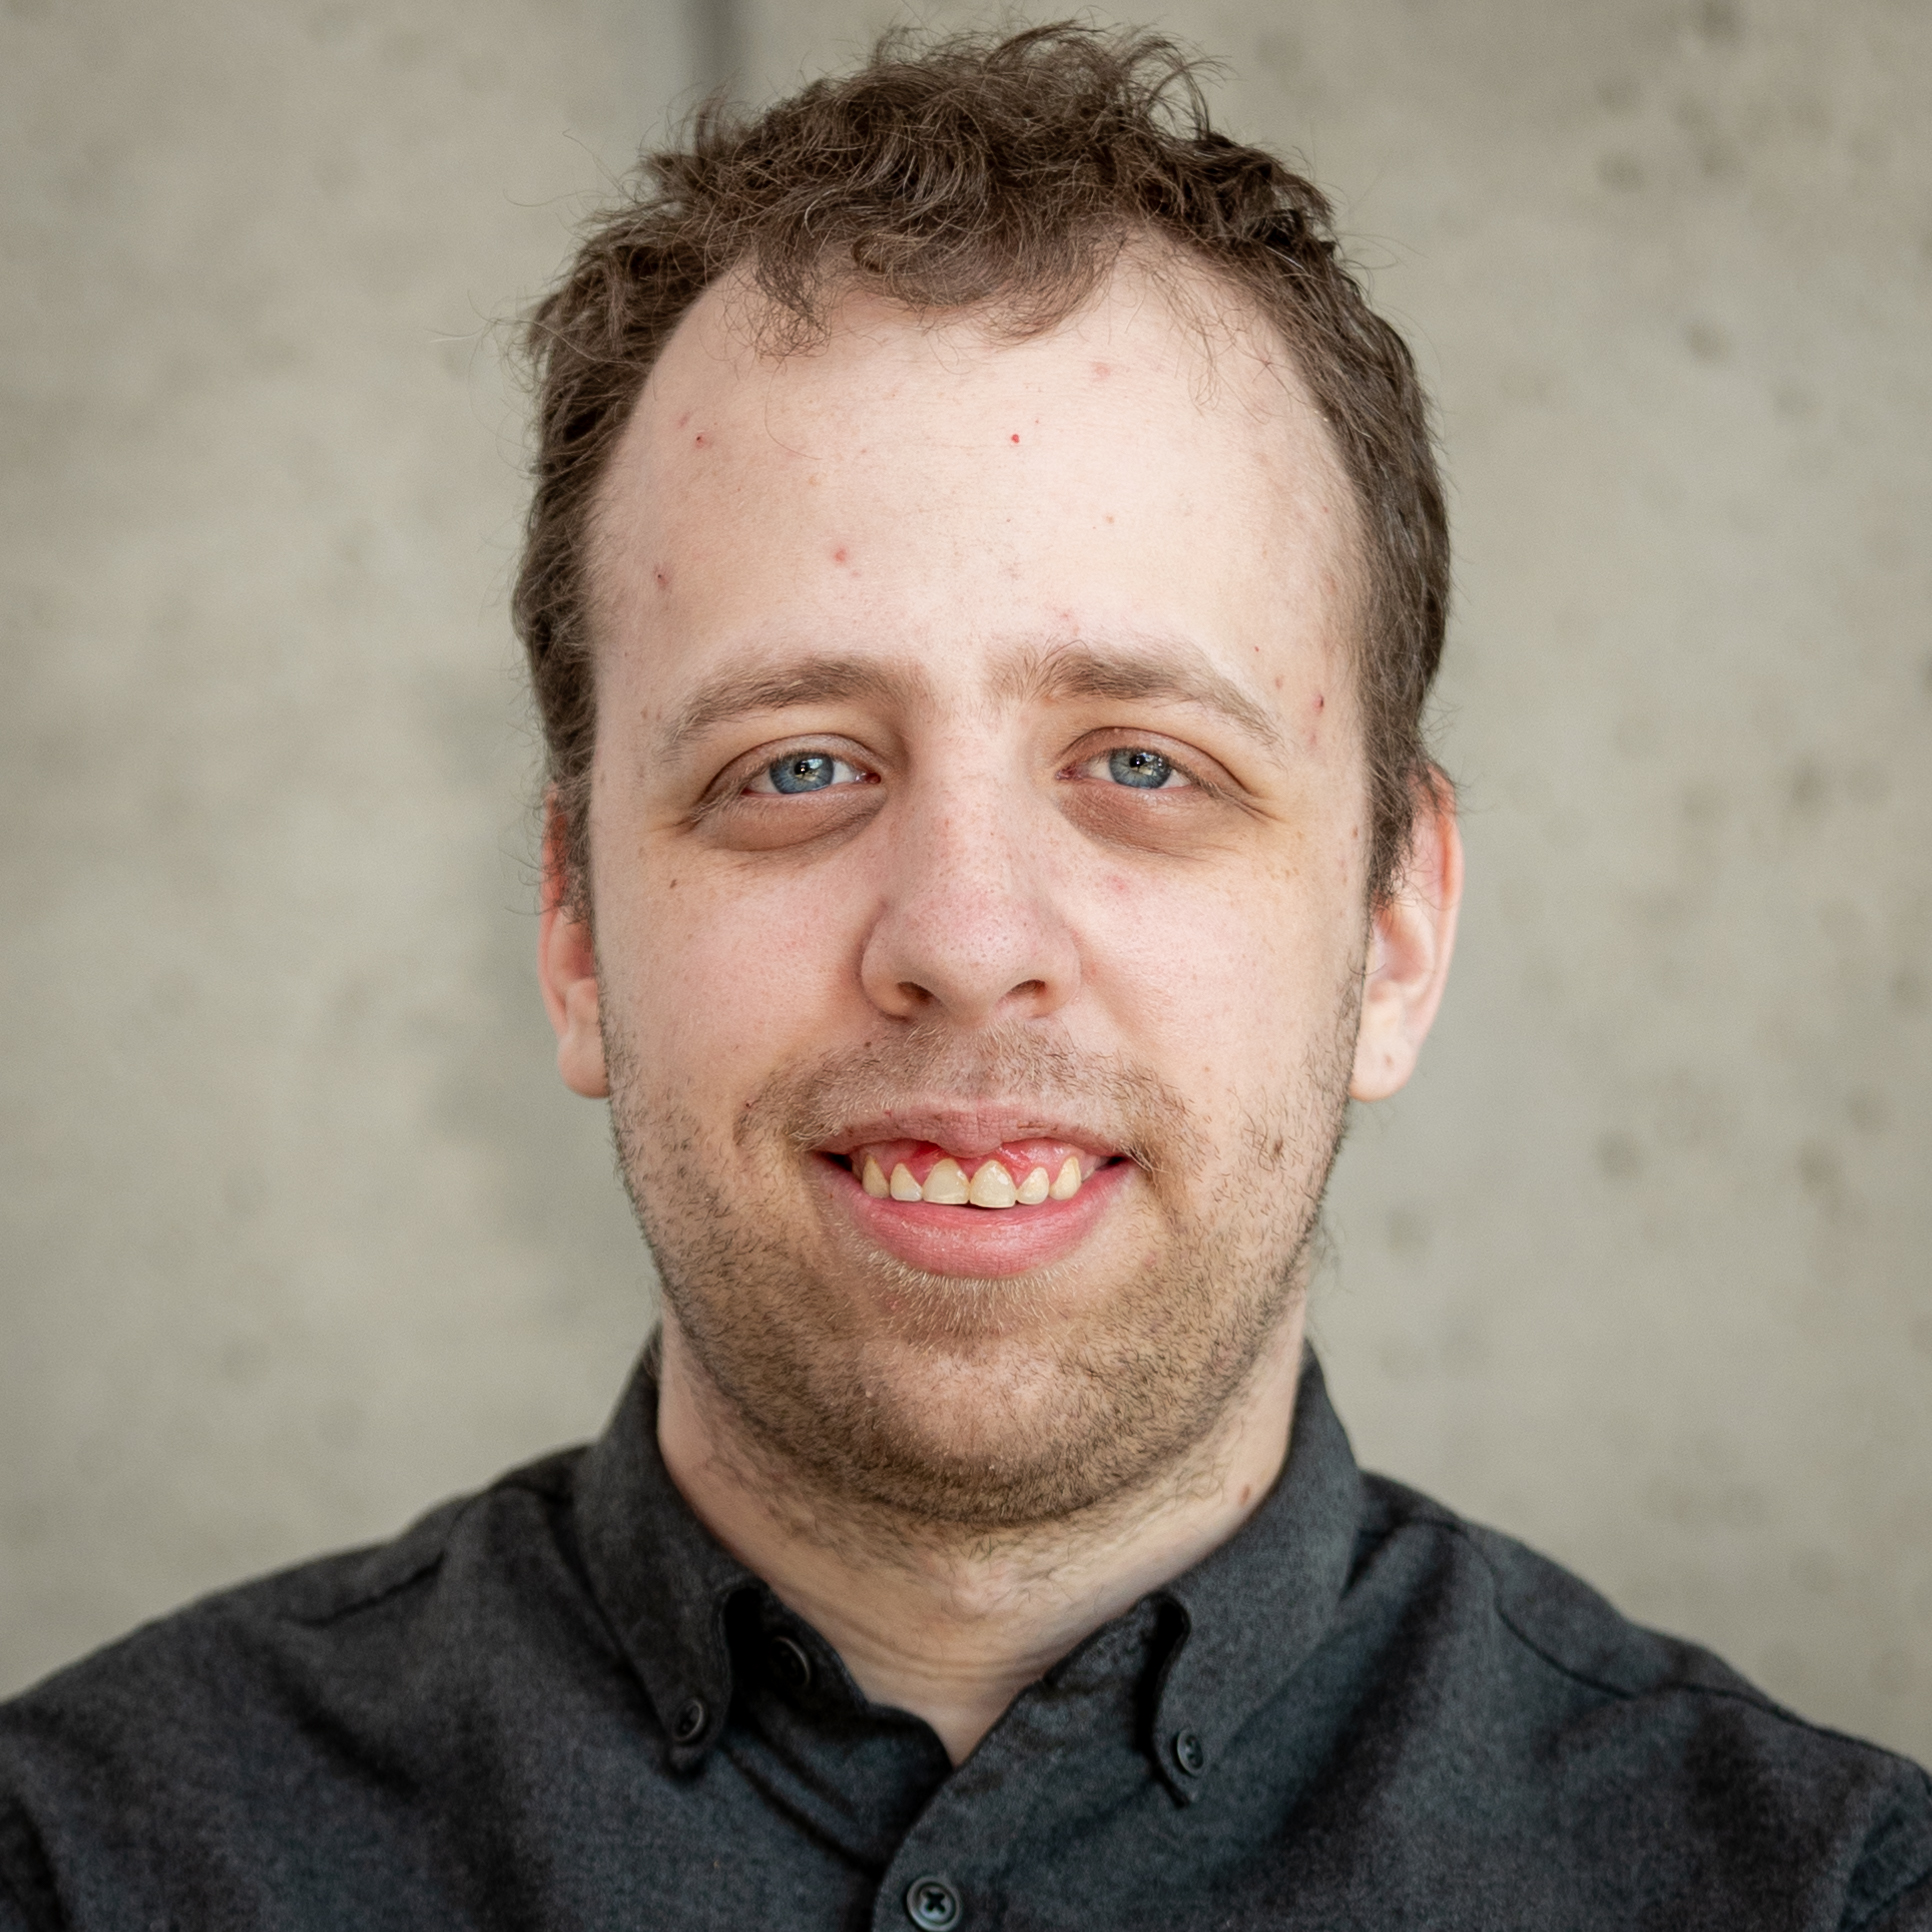
\includegraphics[width=0.9\linewidth]{img/membres/Alexandre-Bergeron-2.jpg} 
\end{wrapfigure}
\subsubsection*{}
\vspace{2mm}
\textbf{Alexandre Bergeron}\\
Télémétrie

\begin{wrapfigure}[5]{r}{0.25\textwidth}
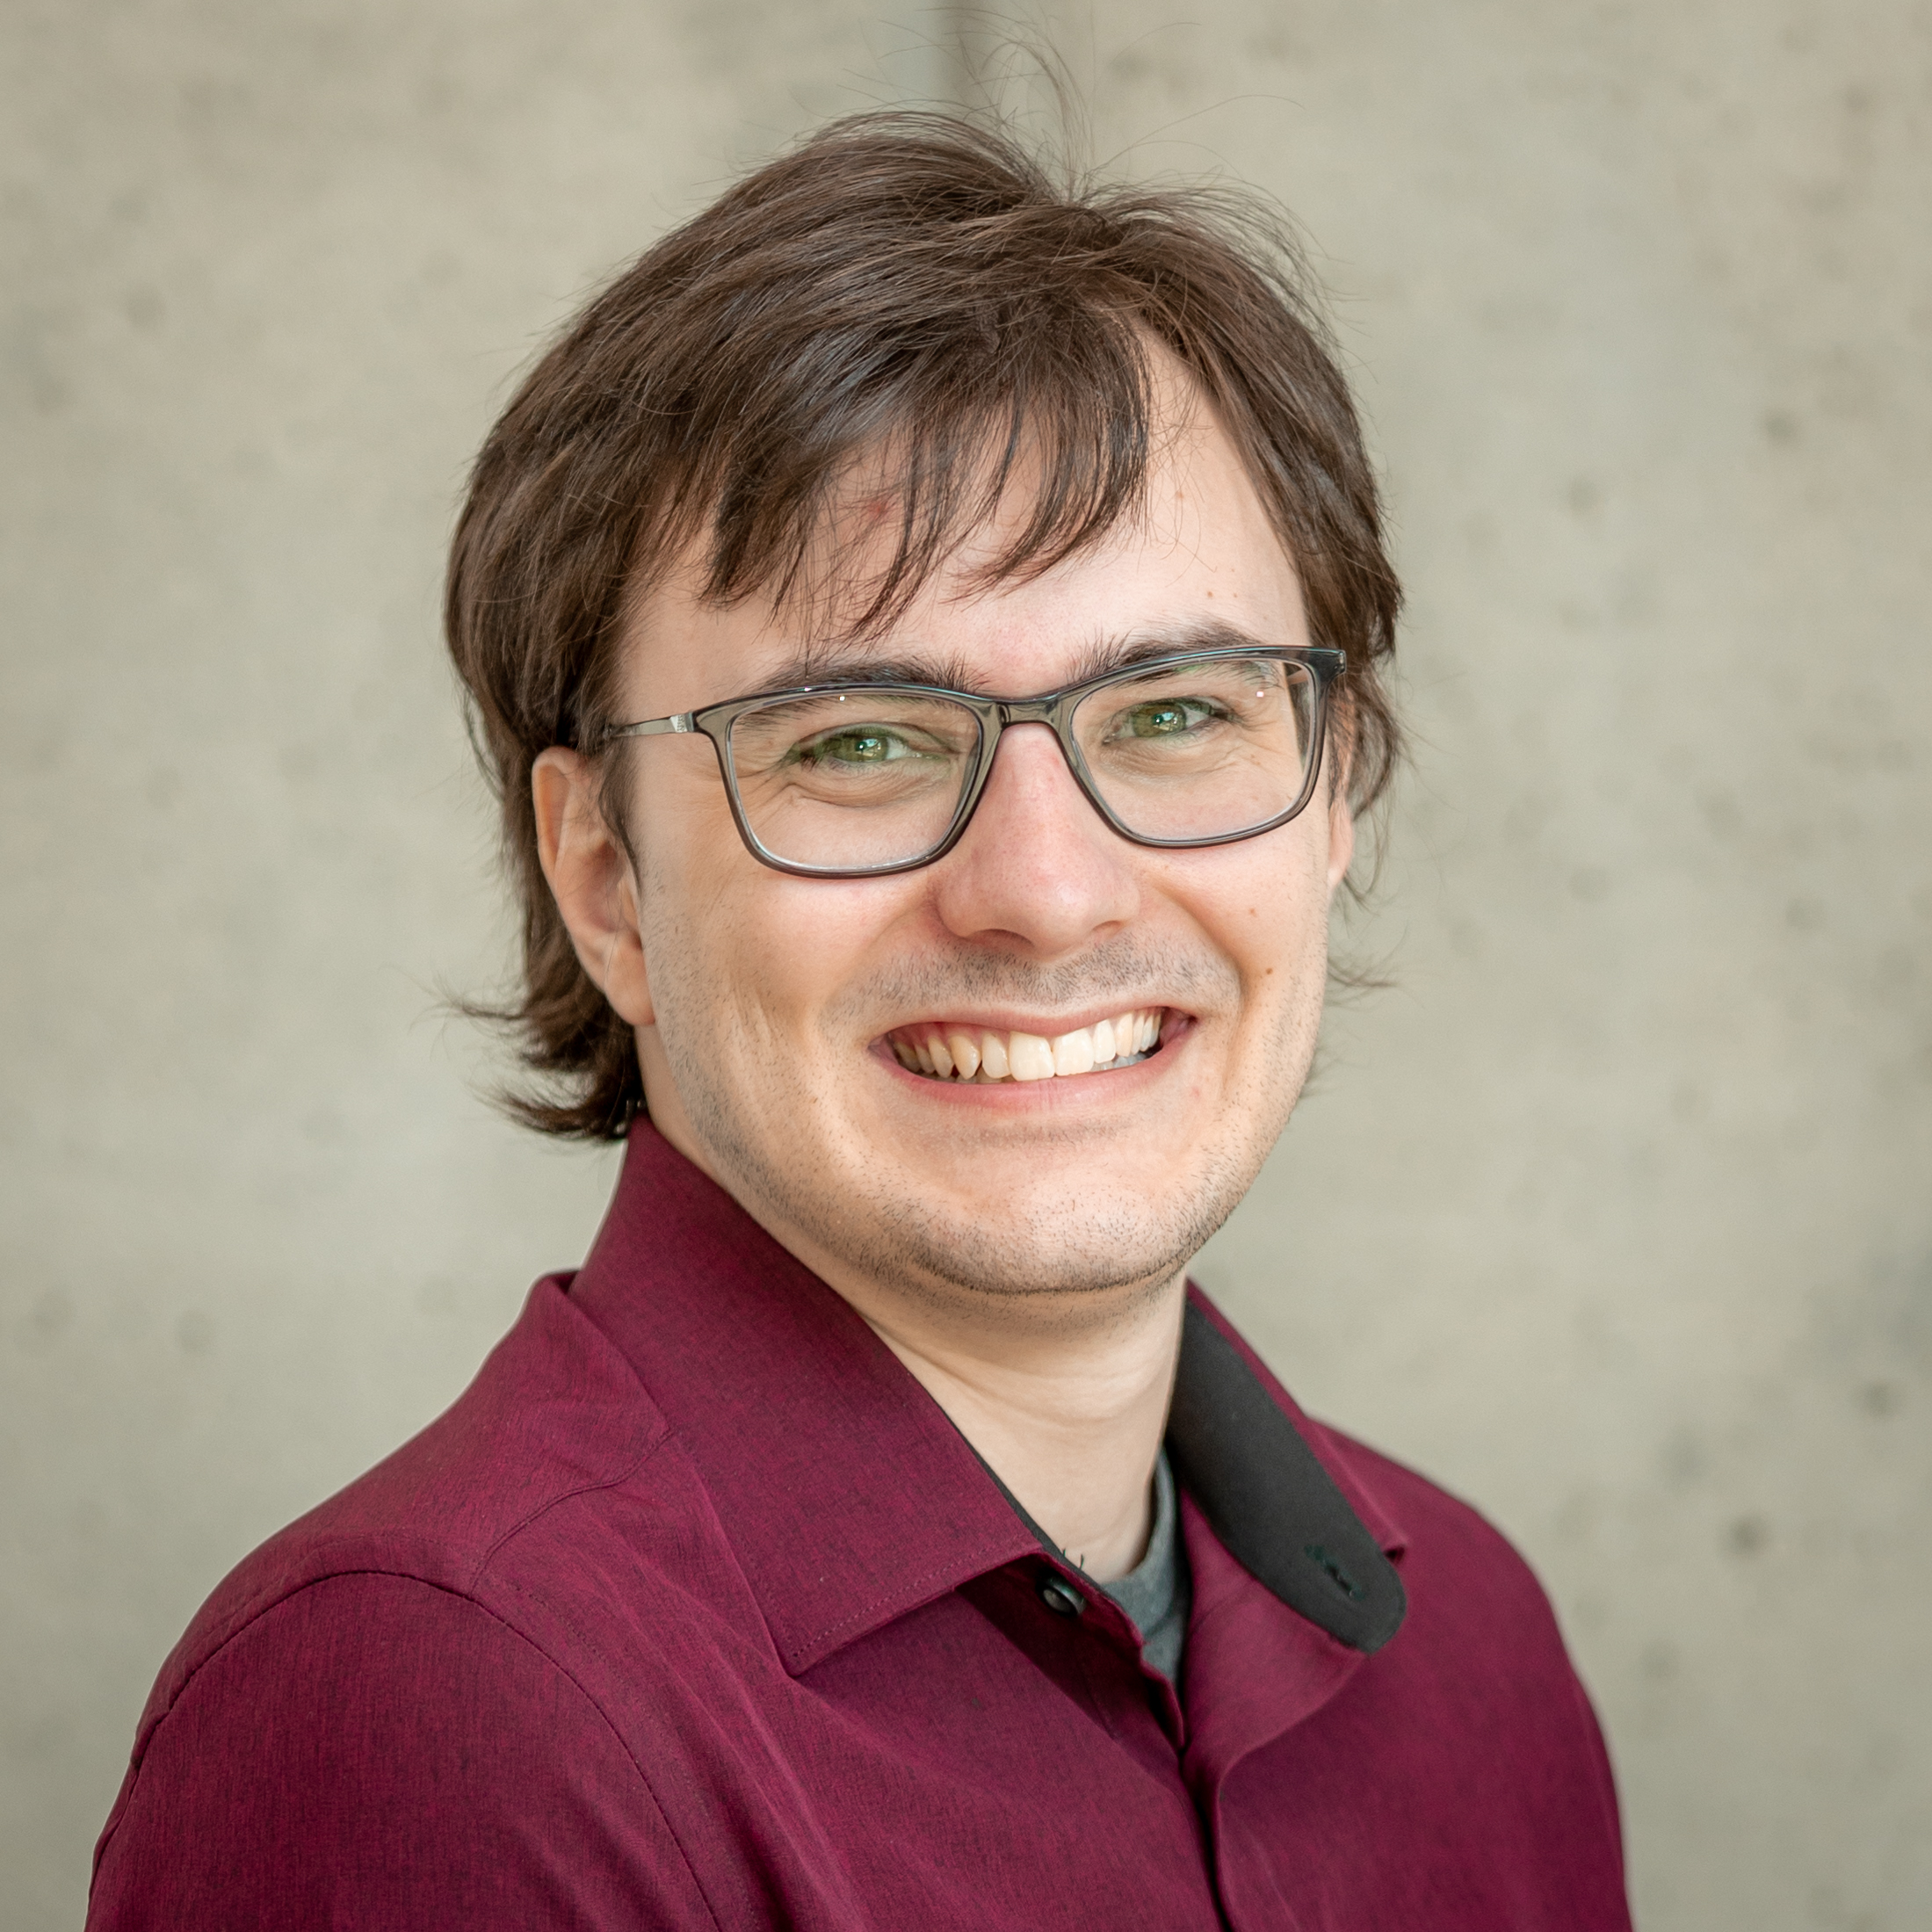
\includegraphics[width=.9\linewidth]{img/membres/Malik-Claveau-2.jpg} 
\end{wrapfigure}
\subsubsection*{}
\vspace{2mm}
\textbf{Malik Claveau}\\
Simulateur

\begin{wrapfigure}[5]{r}{0.25\textwidth}
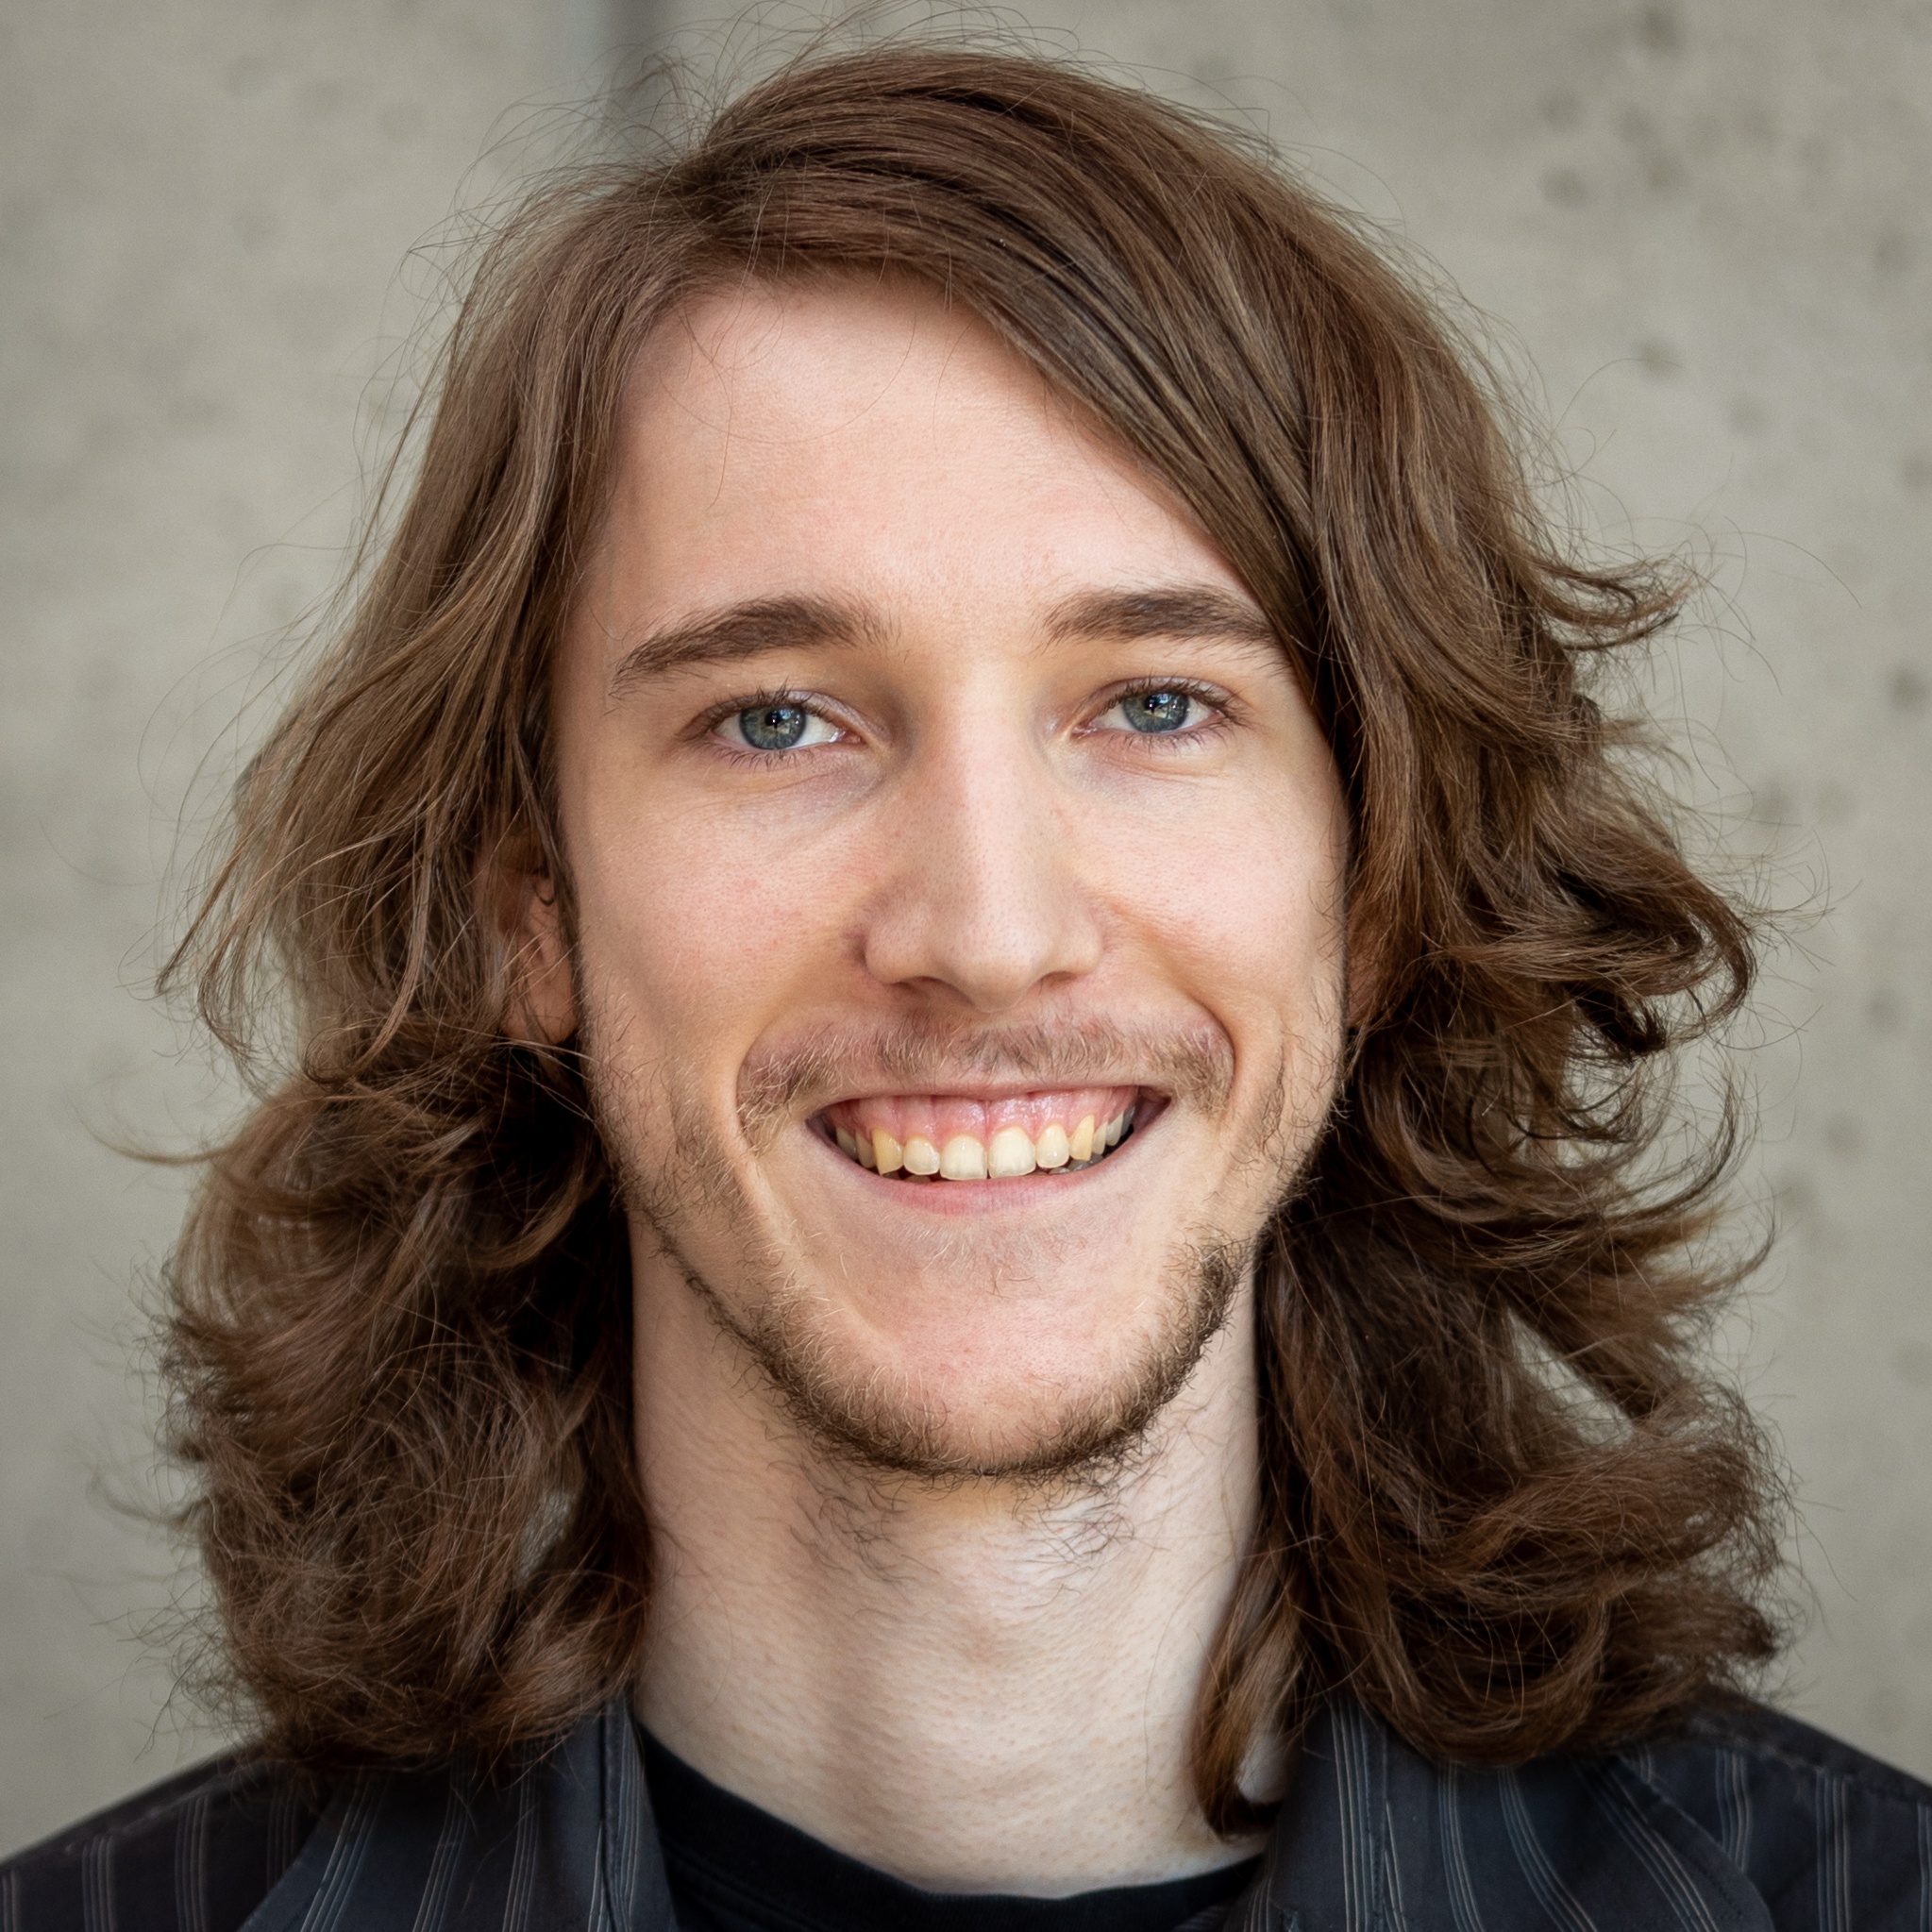
\includegraphics[width=.9\linewidth]{img/membres/Claude-Garrison-Pelletier-2.jpg} 
\end{wrapfigure}
\subsubsection*{}
\vspace{2mm}
\textbf{Claude Garrison-Pelletier}\\
Simulateur

\begin{wrapfigure}[5]{r}{0.25\textwidth}
\includegraphics[width=.9\linewidth]{img/membres/Charles-Étienne-Granger-3.jpg} 
\end{wrapfigure}
\subsubsection*{}
\vspace{2mm}
\textbf{Charles-Étienne Granger}\\
Simulateur/Télémétrie

\begin{wrapfigure}[5]{r}{0.25\textwidth}
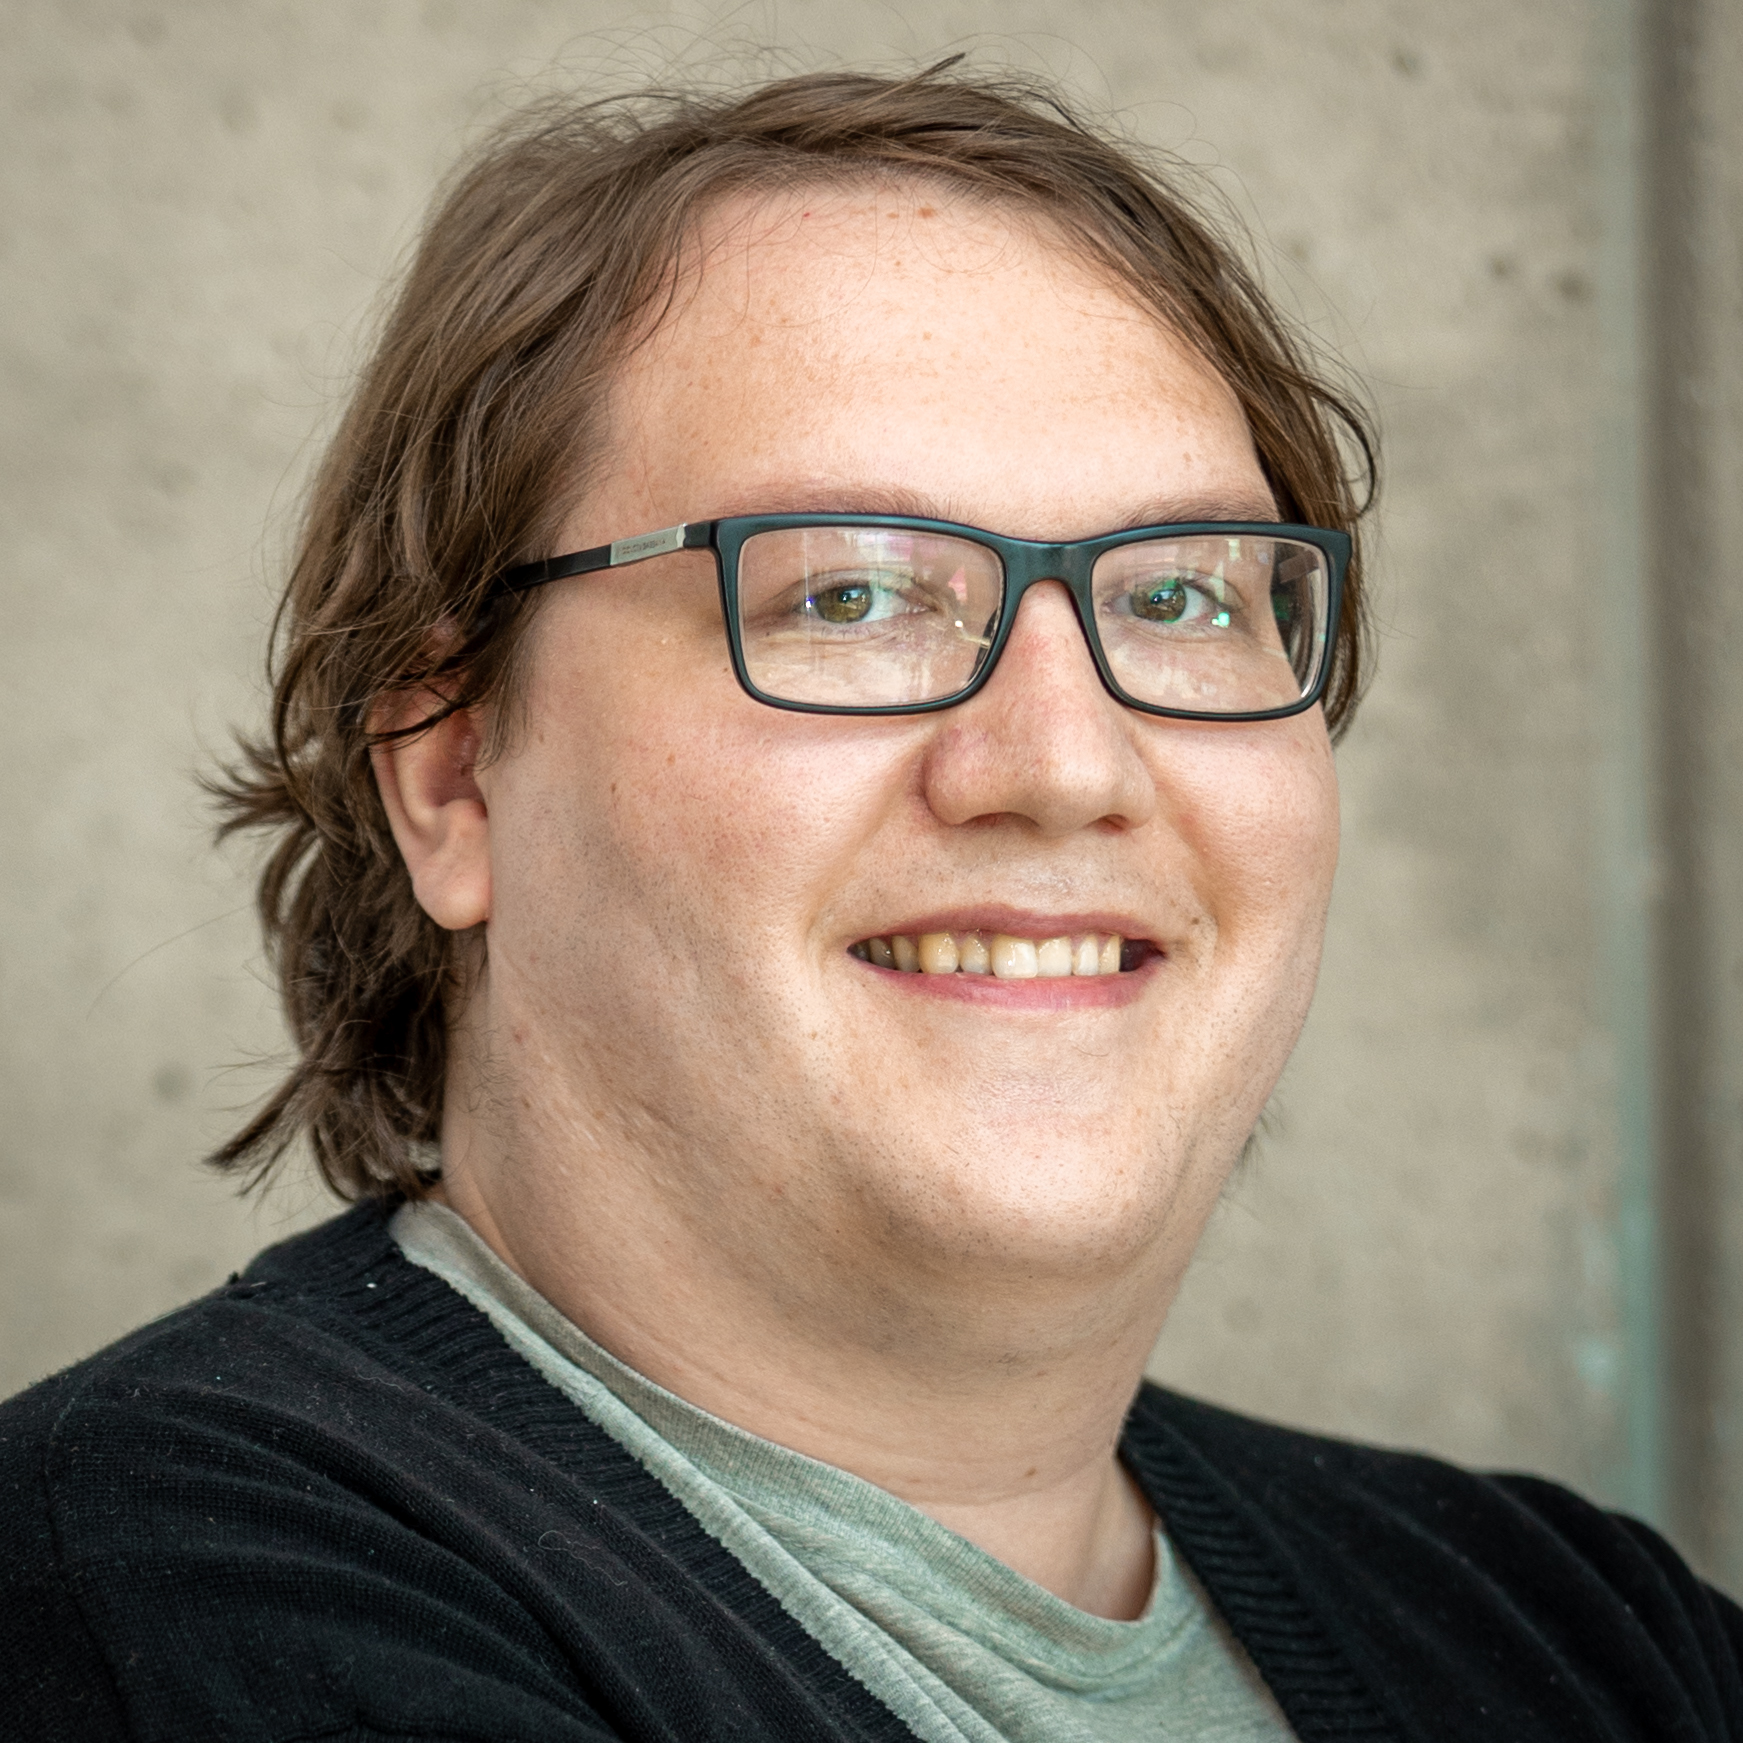
\includegraphics[width=.9\linewidth]{img/membres/Marian-Lambert-Rivest-3.jpg} 
\end{wrapfigure}
\subsubsection*{}
\vspace{2mm}
\textbf{Marian Lambert-Rivest}\\
Simulateur

\begin{wrapfigure}[5]{r}{0.25\textwidth}
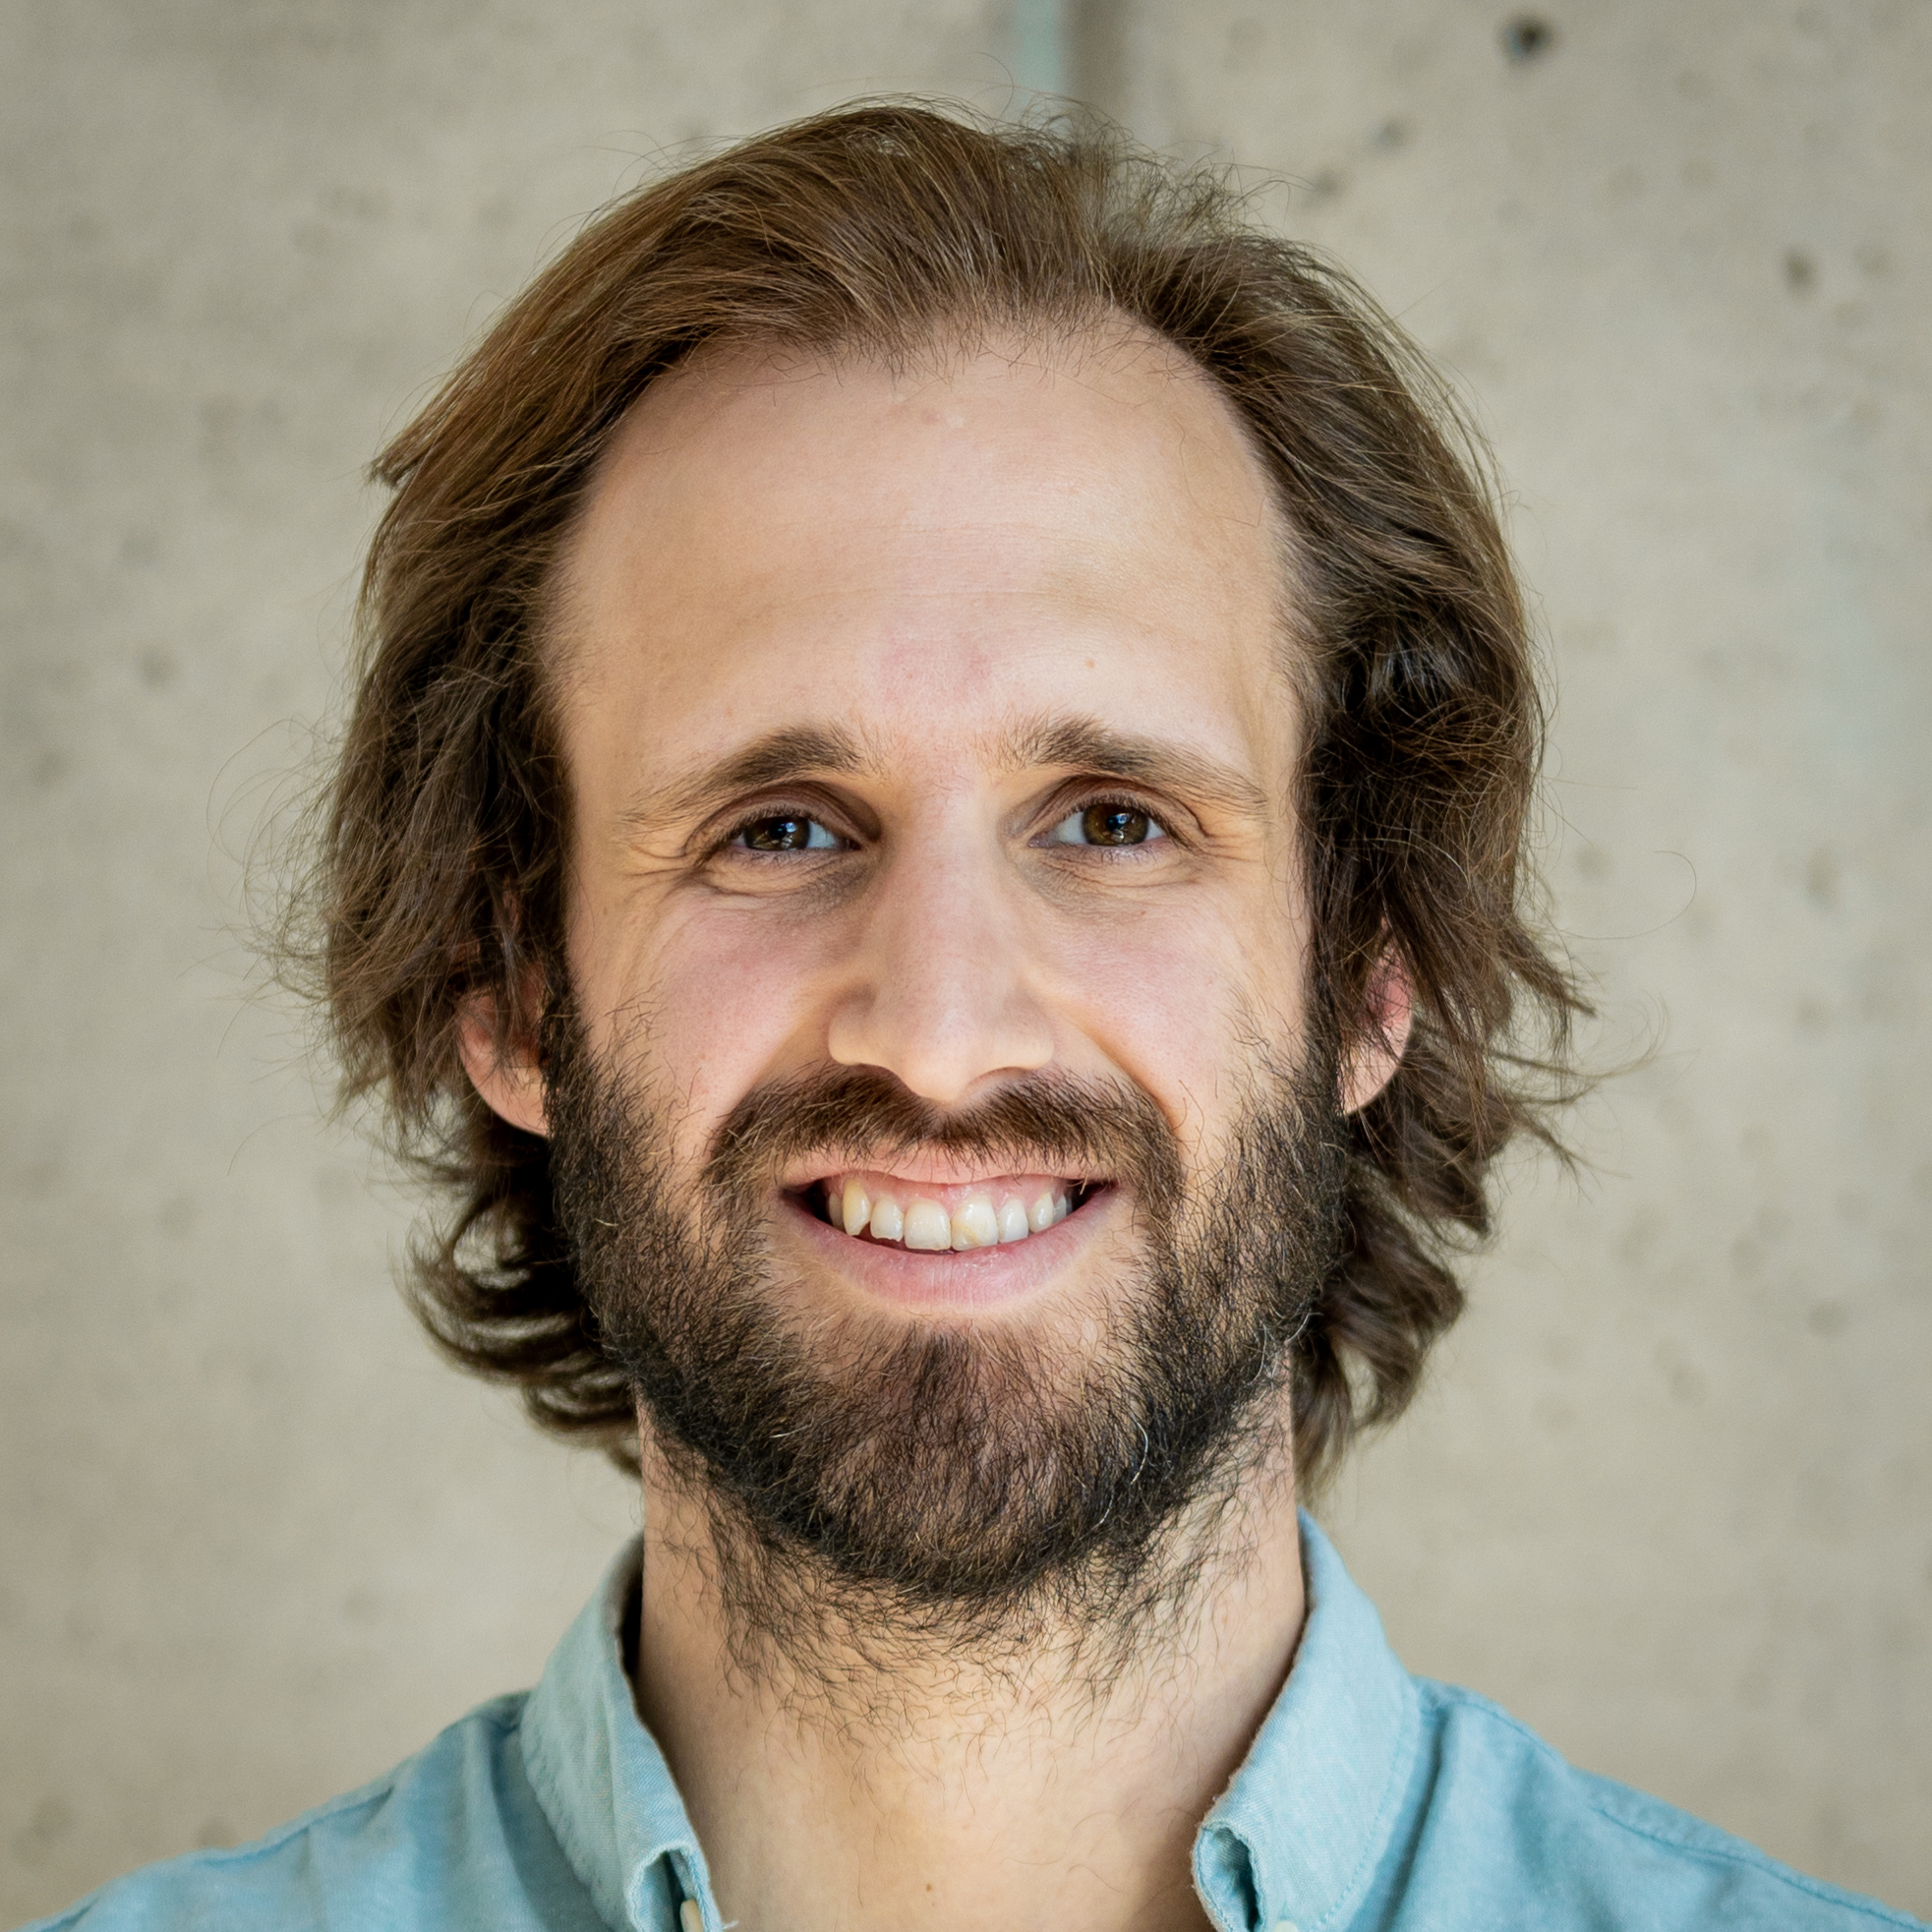
\includegraphics[width=.9\linewidth]{img/membres/Mathieu-Parent-2.jpg} 
\end{wrapfigure}
\subsubsection*{}
\vspace{2mm}
\textbf{Mathieu Parent}\\
Simulateur

\begin{wrapfigure}[5]{r}{0.25\textwidth}
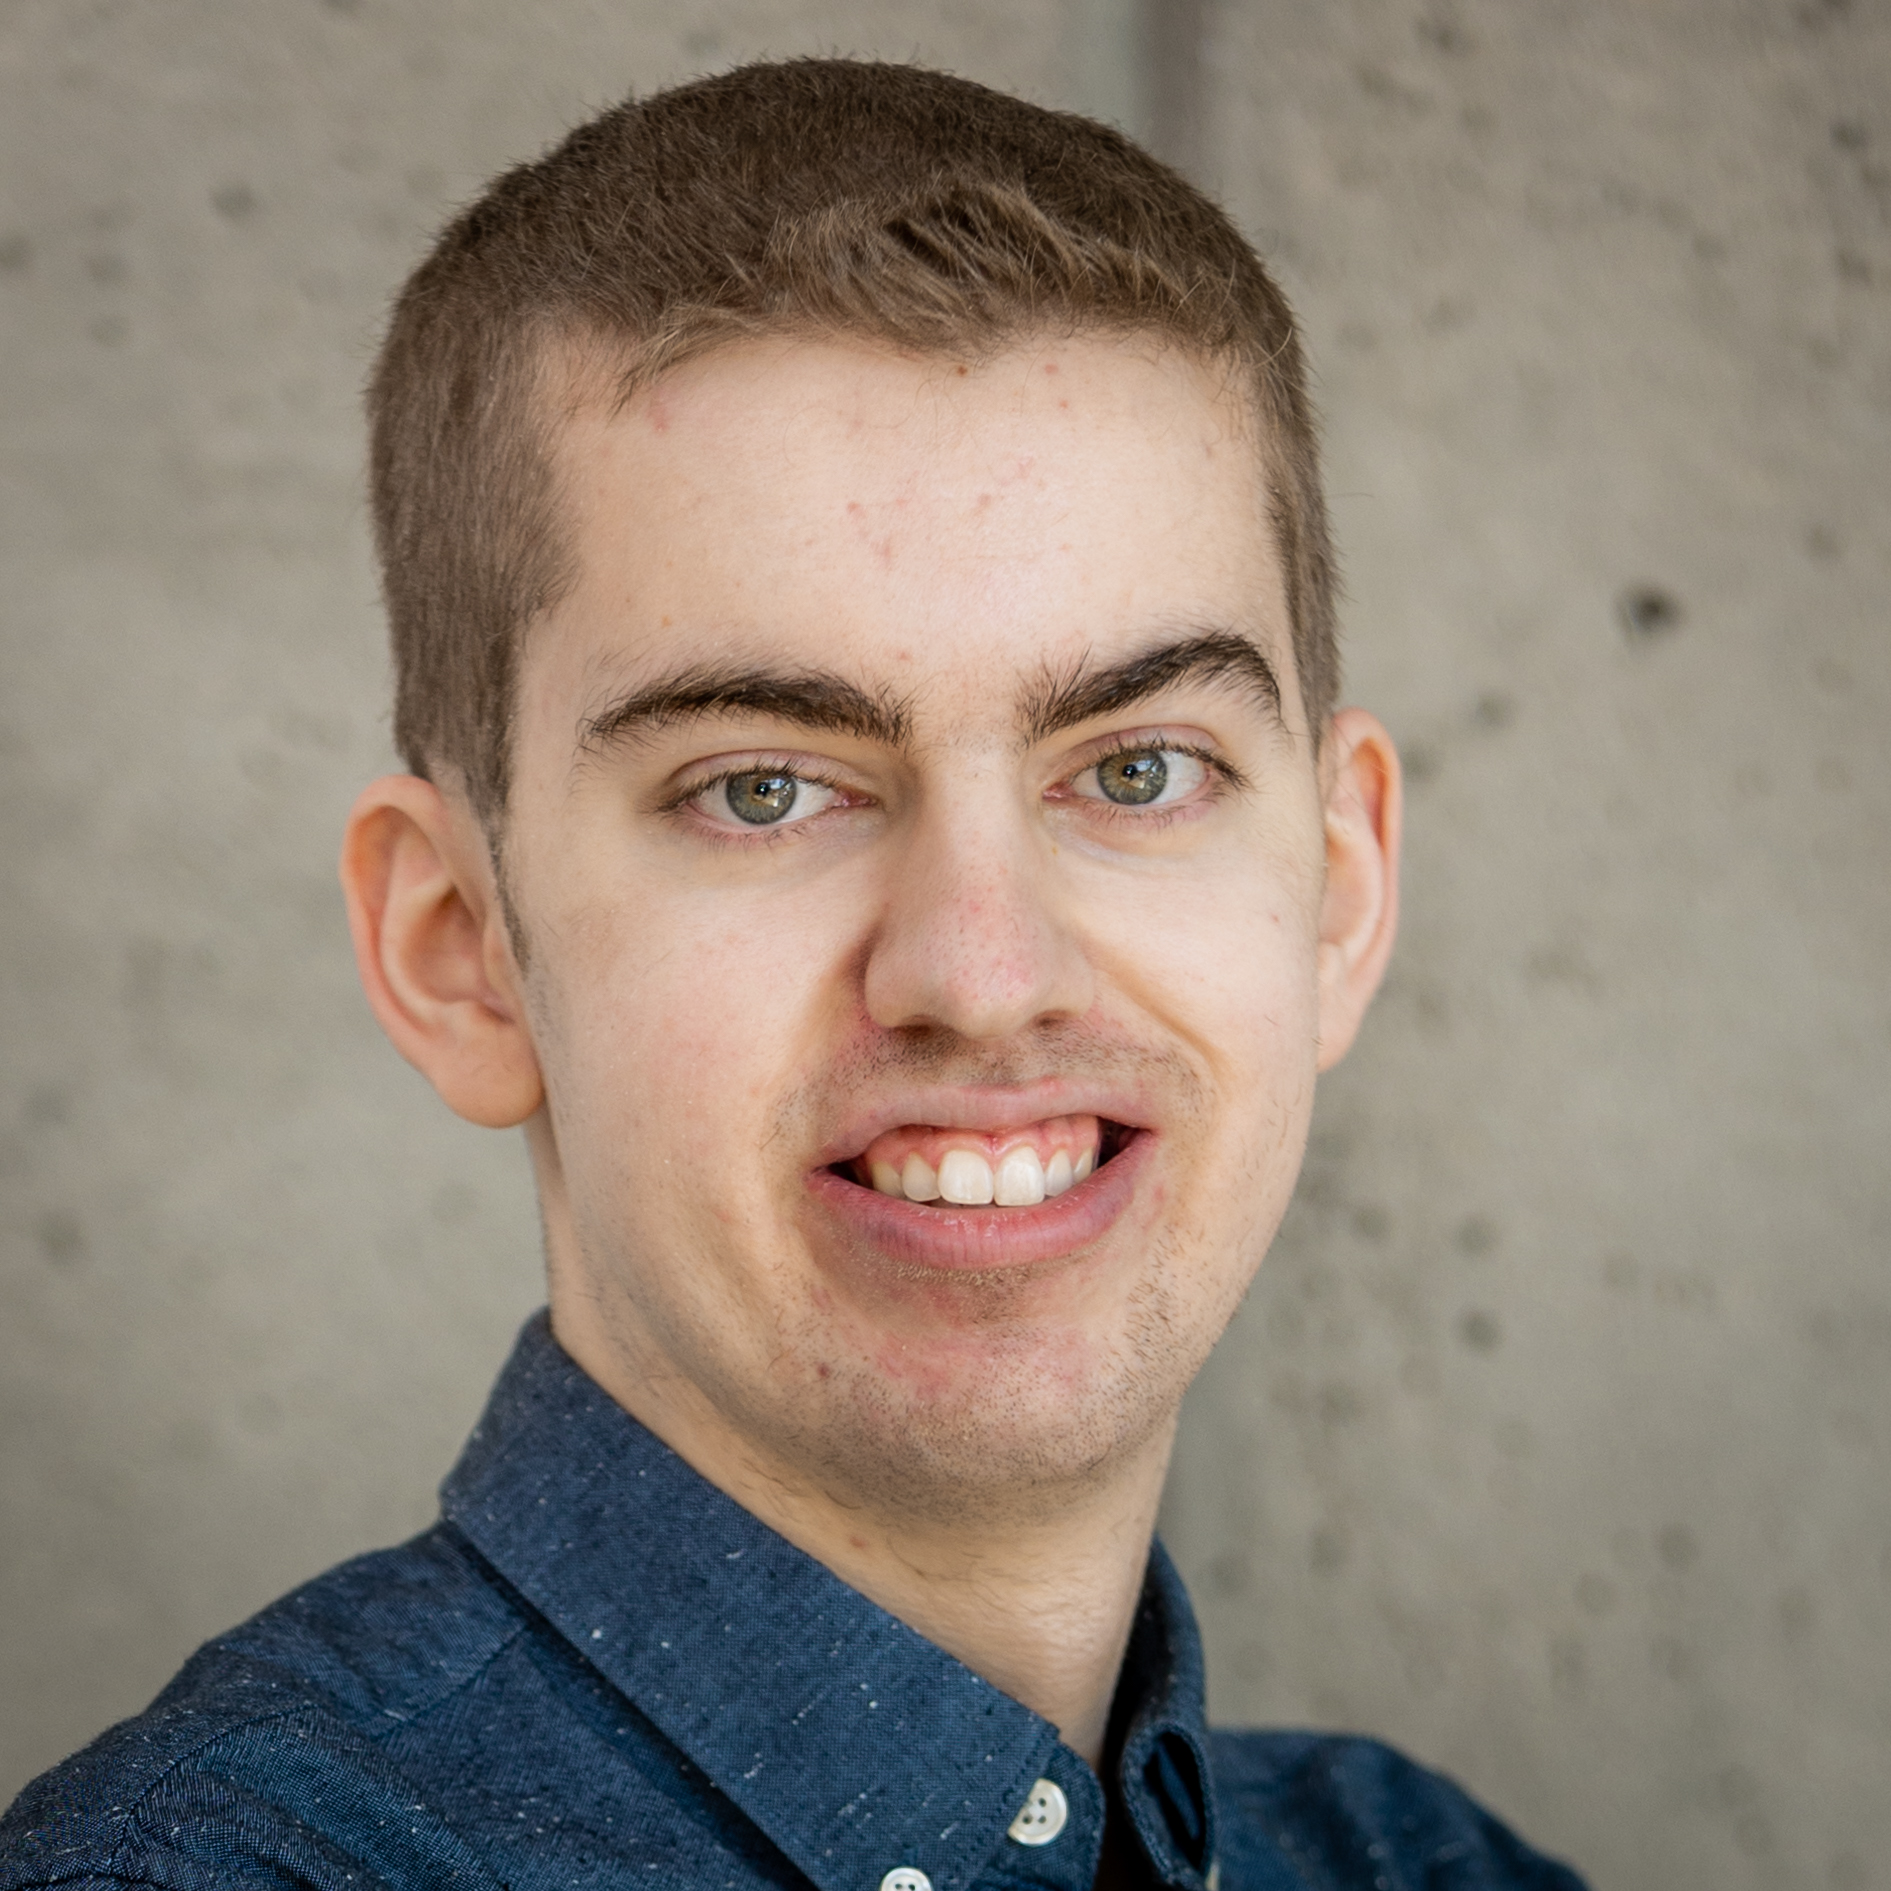
\includegraphics[width=.9\linewidth]{img/membres/Gabriel-Quirion-3.jpg} 
\end{wrapfigure}
\subsubsection*{}
\vspace{2mm}
\textbf{Gabriel Quirion}\\
Contrôle

\begin{wrapfigure}[5]{r}{0.25\textwidth}
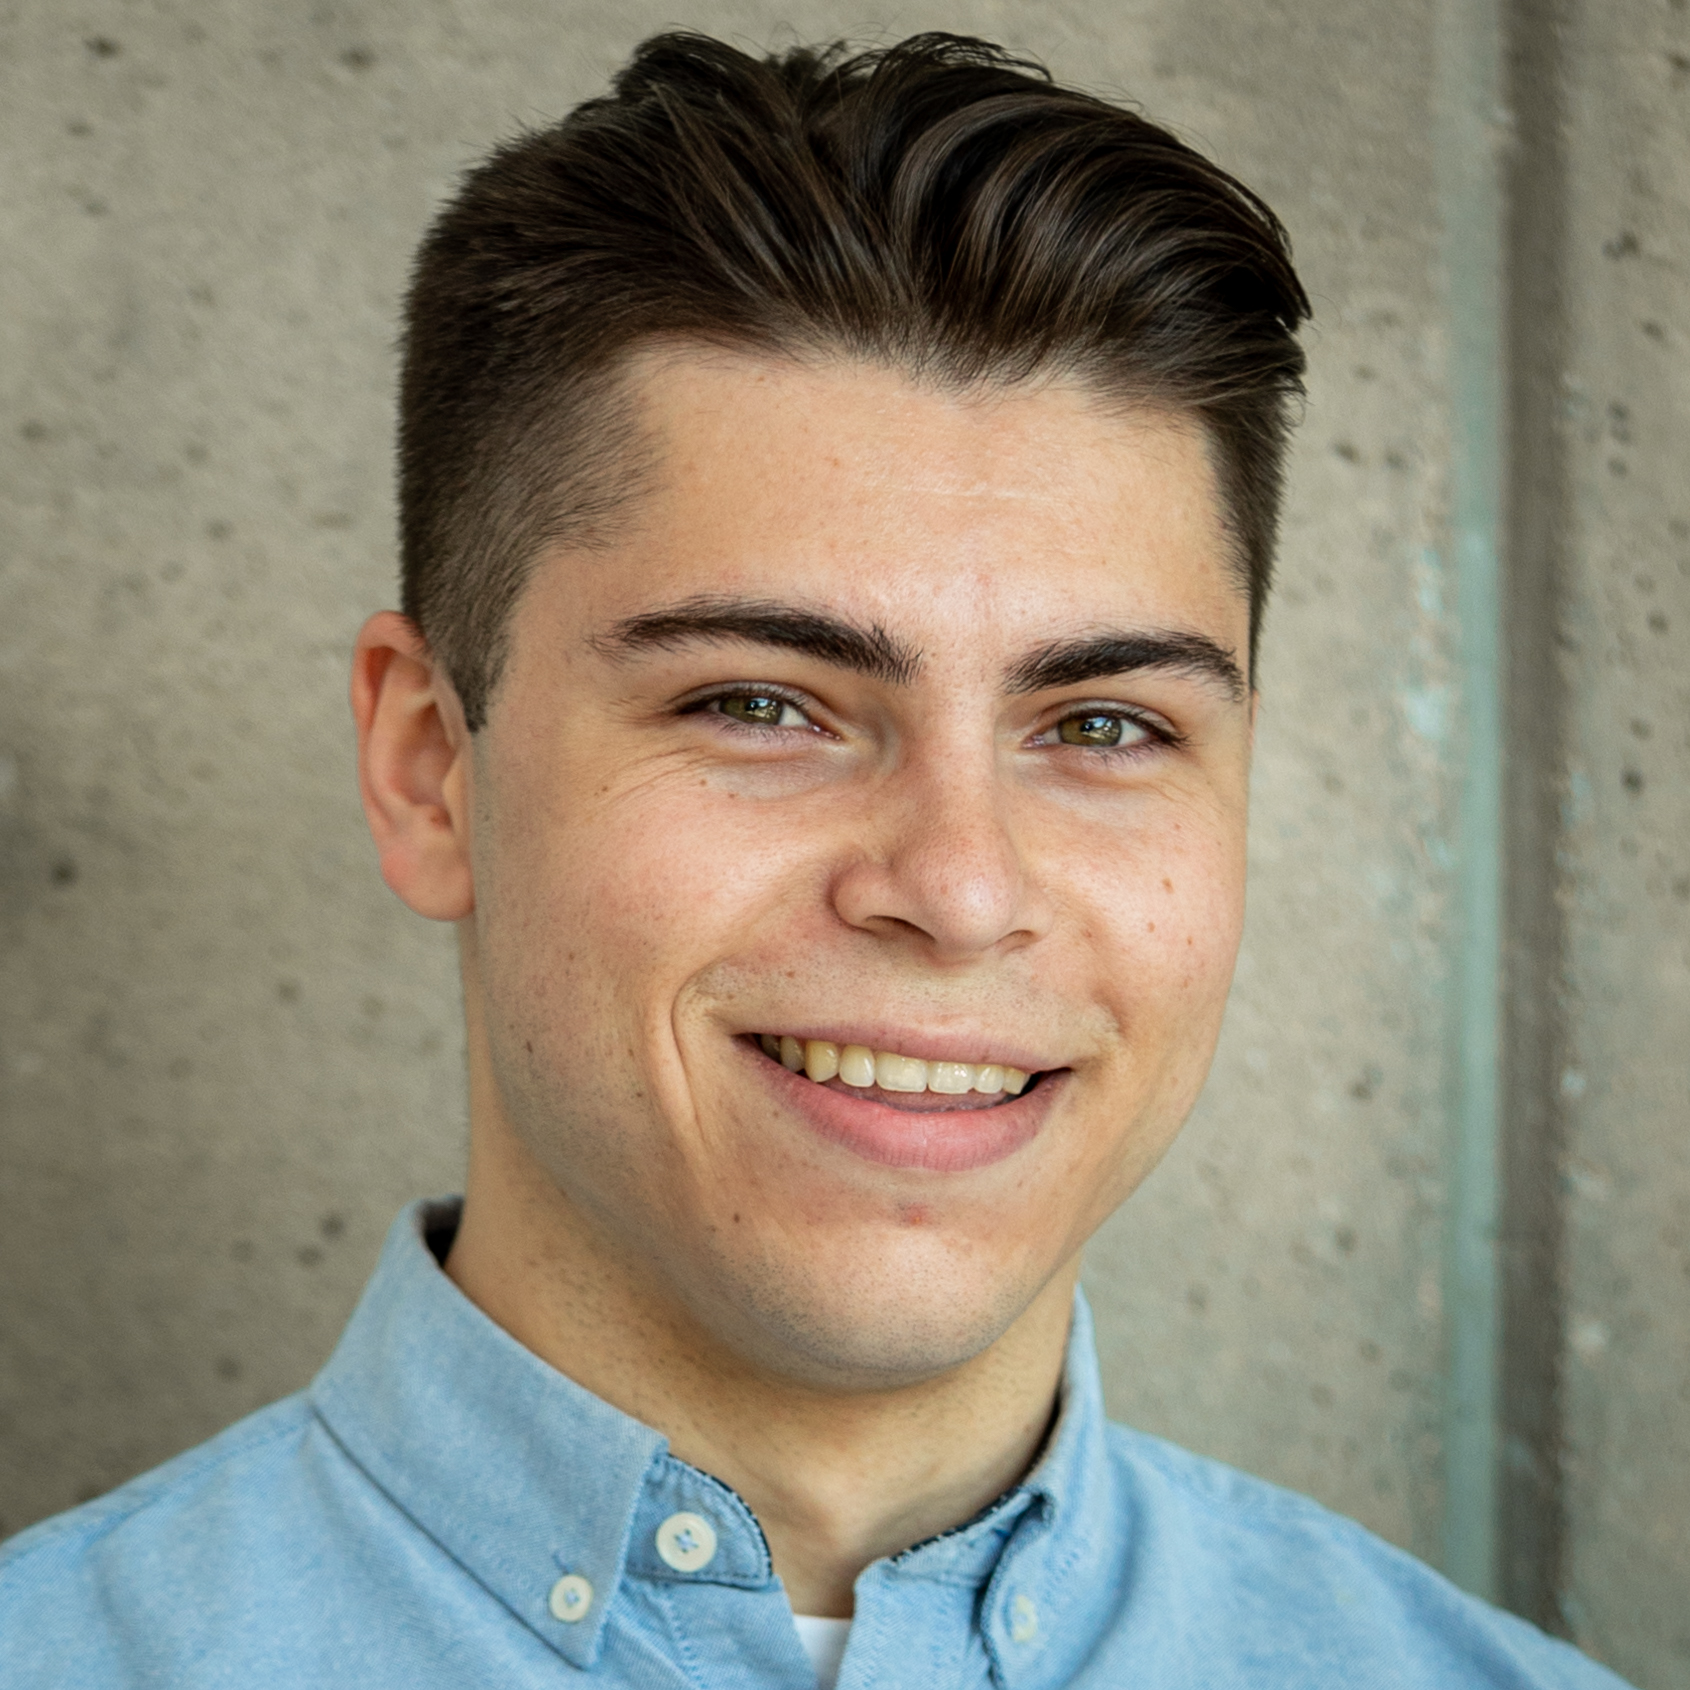
\includegraphics[width=.9\linewidth]{img/membres/William-Rousseau-2.jpg} 
\end{wrapfigure}
\subsubsection*{}
\vspace{2mm}
\textbf{William Rousseau}\\
Simulateur

\begin{wrapfigure}[5]{r}{0.25\textwidth}
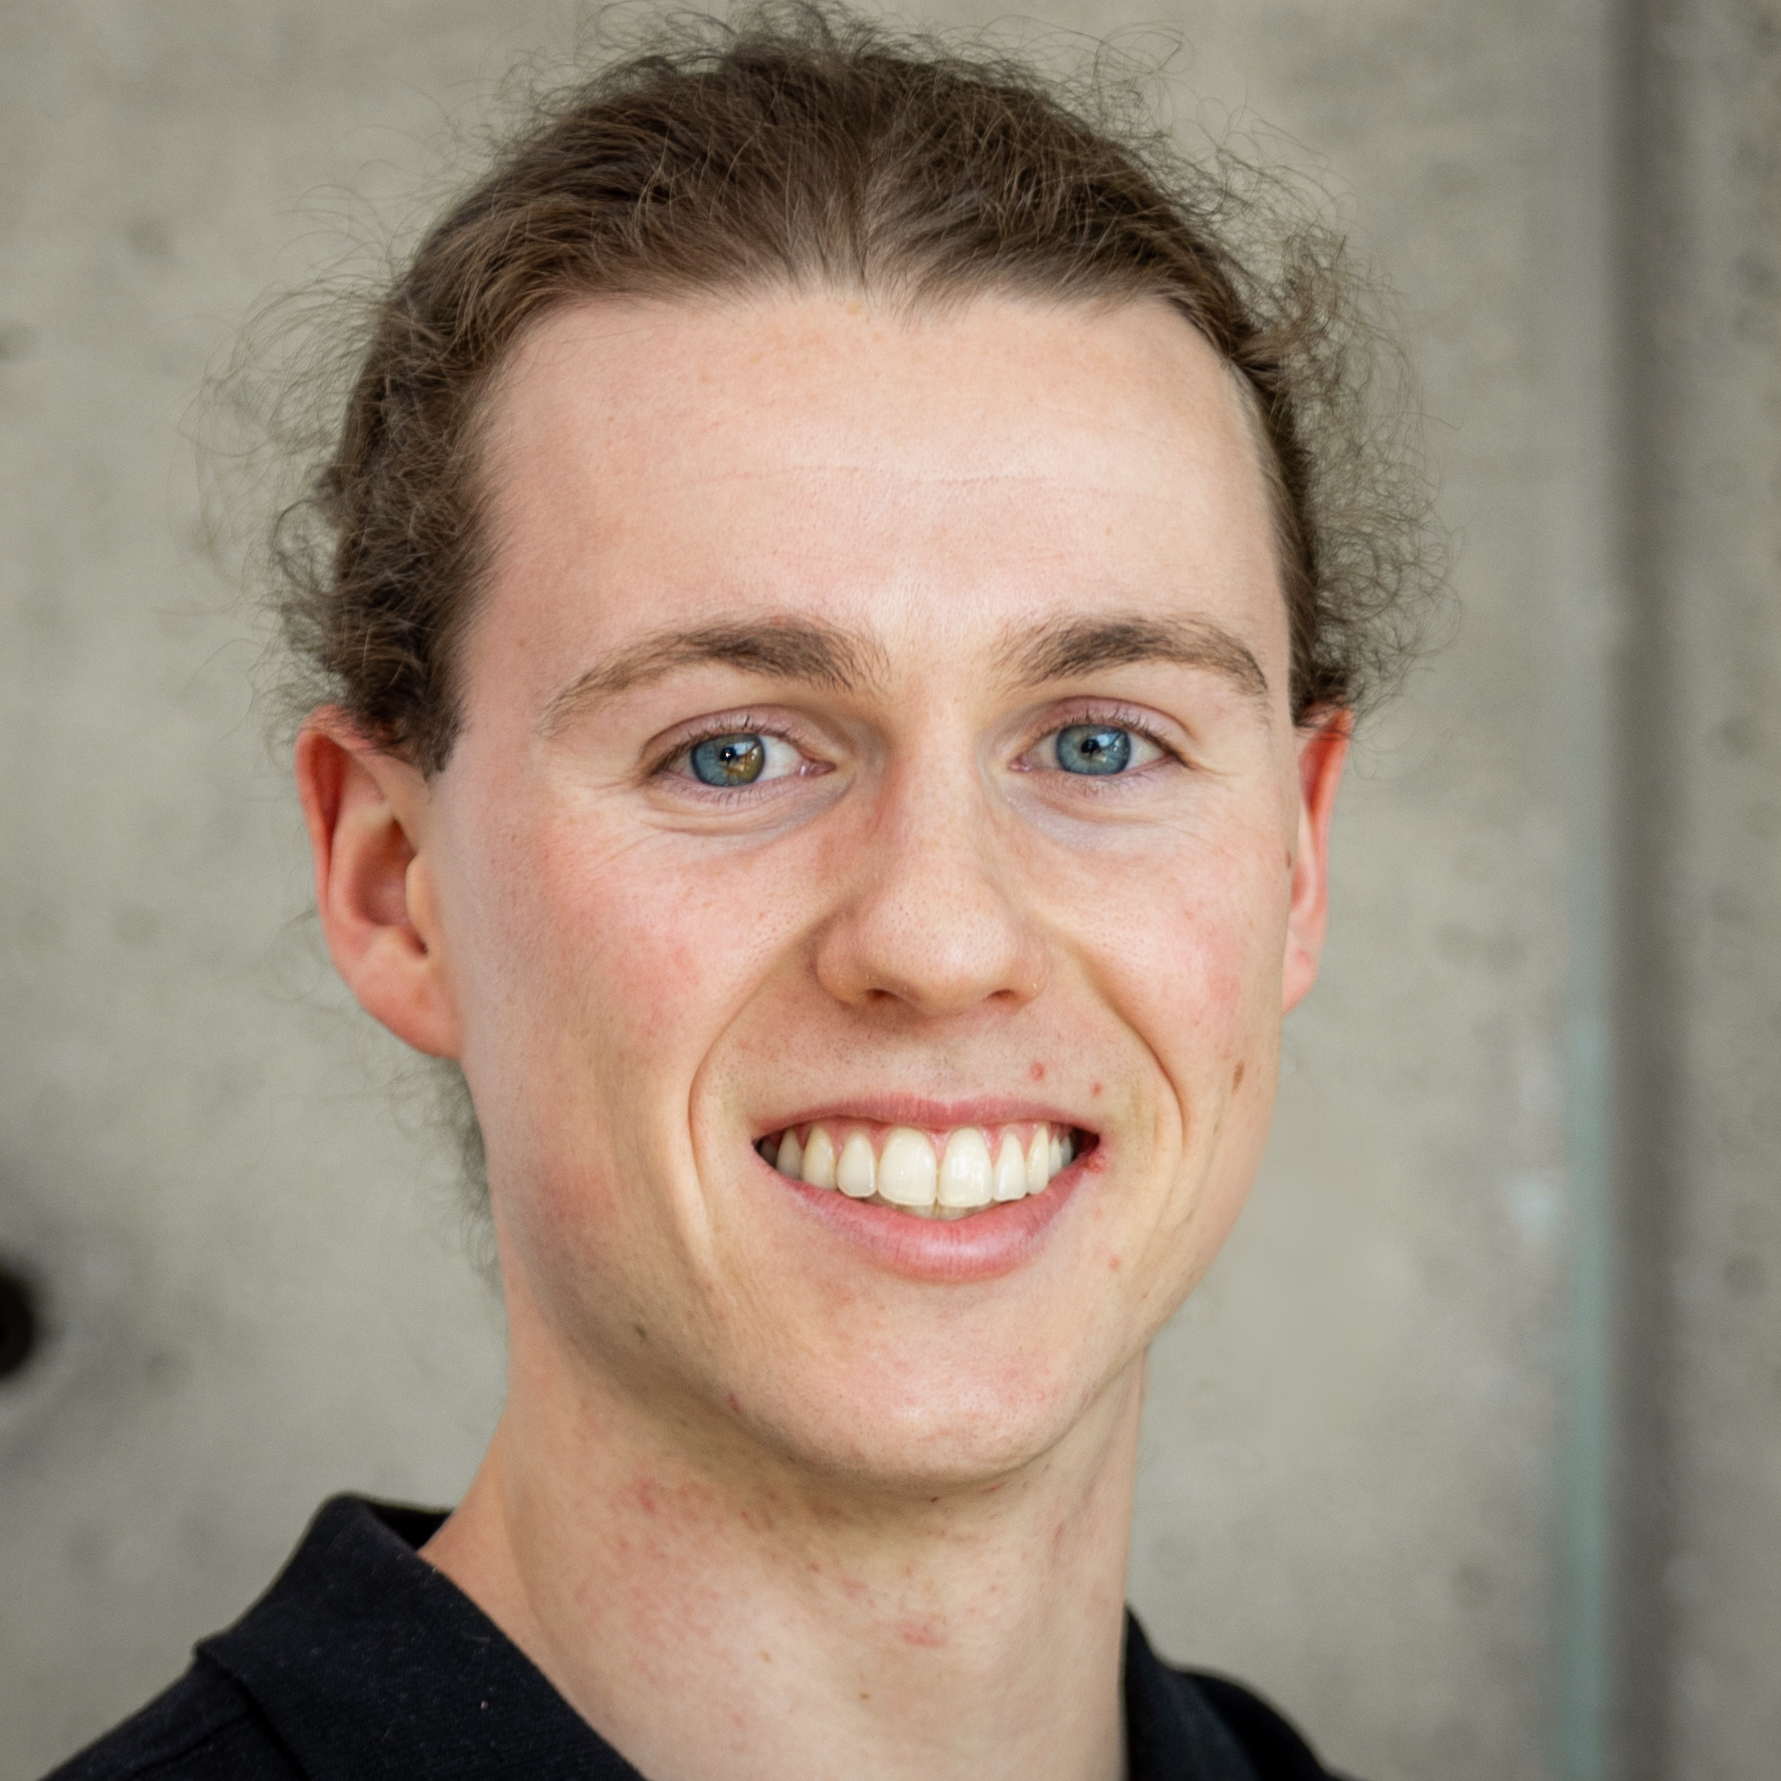
\includegraphics[width=.9\linewidth]{img/membres/Louis-Tardif-3.jpg} 
\end{wrapfigure}
\subsubsection*{}
\vspace{2mm}
\textbf{Louis Tardif}\\
Contrôle
\vspace{1cm}
}


\headerbox{Courbe en S}{name=courbe_s,column=0,span=2,below=objectif_session}{
\hspace{1cm}
\begin{center}
    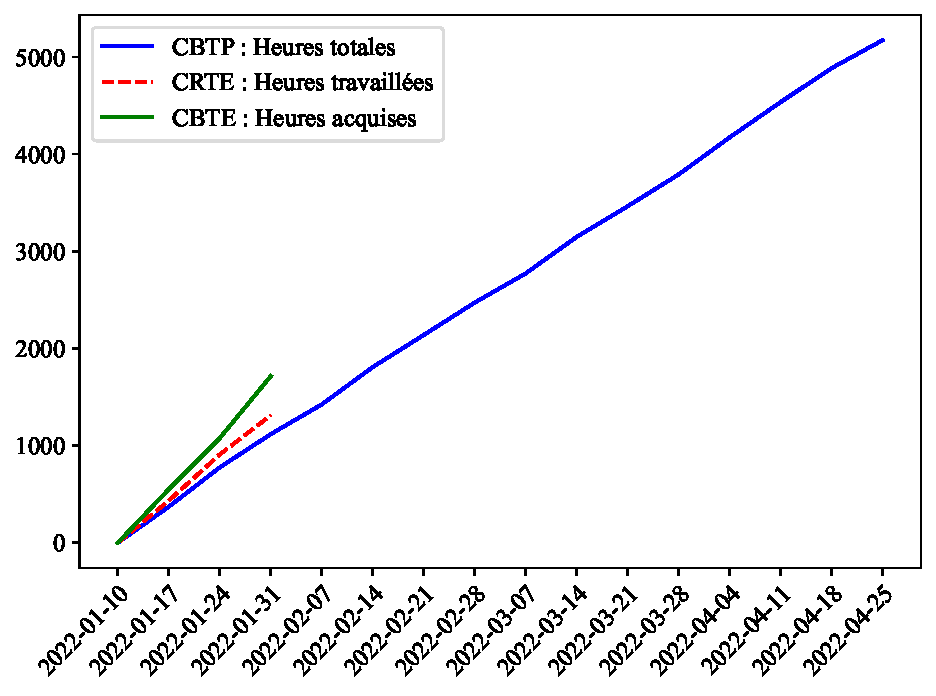
\includegraphics[scale=.54]{img/Courbe_S.pdf}
\end{center}
}

\headerbox{Heures travaillées}{name=heures,column=0,span=2,below=courbe_s}{
\hspace{1cm}
\begin{center}
    \includegraphics[scale=.75]{img/Heures_travaillees.pdf}
\end{center}
}

\headerbox{État du projet}{name=résumé_semaine,column=0,span=2,below=heures}{
\hspace{1cm}
\begin{center}
\begin{itemize}
    \item Simulateur: Il manque seulement seulement de l'intégration pour la v1 du simulateur
    \item Contrôle Moteur: Encore en ligne avec les objectifs
    \item Instrumentation: Communication avec les autres équipes pour établir les besoins et ce qui est déjà établi.
\end{itemize}
\end{center}

}

\end{poster}

\begin{poster}
{
grid=false,
headerborder=open, % Adds a border around the header of content boxes
colspacing=1em, % Column spacing
bgColorOne=white, % Background color for the gradient on the left side of the poster
bgColorTwo=white, % Background color for the gradient on the right side of the poster
borderColor=Mycolor1, % Border color
headerColorOne=Mycolor2, % Background color for the header in the content boxes (left side)
headerColorTwo=Mycolor2, % Background color for the header in the content boxes (right side)
headerFontColor=white, % Text color for the header text in the content boxes
boxColorOne=white, % Background color of the content boxes
textborder=rounded, %rectangle, % Format of the border around content boxes, can be: none, bars, coils, triangles, rectangle, rounded, roundedsmall, roundedright or faded
eyecatcher=false, % Set to false for ignoring the left logo in the title and move the title left
headerheight=0\textheight, % Height of the header
headershape=rounded, % Specify the rounded corner in the content box headers, can be: rectangle, small-rounded, roundedright, roundedleft or rounded
headershade=plain,
headerfont=\Large\textsf, % Large, bold and sans serif font in the headers of content boxes
%textfont={\setlength{\parindent}{1.5em}}, % Uncomment for paragraph indentation
linewidth=1pt % Width of the border lines around content boxes
}
{}
{\textsf{{}}} % Titre vide pcq sinon ça plante
\hfill \break % Ligne vide pcq sinon ça plante

\headerbox{Objectifs bimensuels}{name=objectifs,column=0, row=0, span=3}{{\textbf{\large Contrôle Moteur / BMS}\\
\begin{tabularx}{\linewidth}{
    |>{\hsize=0.33\hsize}X|
    >{\hsize=0.33\hsize}X|
    >{\hsize=0.33\hsize}X|
    >{\hsize=2.5\hsize}X|% 10% of 4\hsize 
    >{\hsize=0.5\hsize}X|% 30% of 4\hsize
       % sum=0.2\hsize for 4 columns
  }
    \hline
    \textbf{Planifié(\%)} & \textbf{Progrès(\%)} & \textbf{Planifié(H)} &\textbf{Objectif} & \textbf{Responsable} \\\hline
    50\% & 50\% & 30 & Refactor en correction des calculs FOC & Louis T.\\\hline
    25\% & 25\% & 40 & Tester la prise de mesures et le "tuning" avec STM32CubeMonitor & Louis T.\\\hline
    20\% & 20\% & 10 & Avoir un code qui permet de tester le moteur sur le dynamomètre & Gabriel Q.\\\hline
\end{tabularx}
\newline

\hfill \break
\textbf{\large Simulateur}
\\
\begin{tabularx}{\linewidth}{
    |>{\hsize=0.33\hsize}X|
    >{\hsize=0.33\hsize}X|
    >{\hsize=0.33\hsize}X|
    >{\hsize=2.5\hsize}X|% 10% of 4\hsize 
    >{\hsize=0.5\hsize}X|% 30% of 4\hsize 
       % sum=0.2\hsize for 4 columns 
  }
    \hline
    \textbf{Planifié(\%)} & \textbf{Progrès(\%)} & \textbf{Planifié(H)} &\textbf{Objectif} & \textbf{Responsable} \\\hline
        100\% & 100\% & 14 &  \st{Format data pour logiciel Mtest-7} & Malik C.\\\hline
        100 \% & 100\% & 10 &  \st{Validation format data sur dyno.} & Malik C.\\\hline
        0 \% & 0\% & 12 &  Création script pour sortir torque en fonction RPM de datasheet. & Malik C.\\\hline
        0 \% & 0\% & 0 &  Intégration du parcours sur le dyno de Pascal Messier. & Malik C.\\\hline % nouveau stuff
        100\% & 100\% & 18 &  \st{Rendre la modification des paramêtres plus intuitif} & Mathieu P.\\\hline % Claude 2022-09-21
        75\% & 60\% & 12 &  Véhicule fait des arrêts (stratégie de conduite) & Claude G.-P.\\\hline % Claude 2022-09-21
        100\% & 75\% & 16 &  décélération/acélération dans les virages (stratégie de conduite) & Mathieu P. \\\hline % ?

\end{tabularx}\\

\hfill \break
\textbf{\large Instrumentation}\\
\begin{tabularx}{\linewidth}{
    |>{\hsize=0.33\hsize}X|
    >{\hsize=0.33\hsize}X|
    >{\hsize=0.33\hsize}X|
    >{\hsize=2.5\hsize}X|% 10% of 4\hsize 
    >{\hsize=0.5\hsize}X|% 30% of 4\hsize
       % sum=0.2\hsize for 4 columns
  }
    \hline
    \textbf{Planifié(\%)} & \textbf{Progrès(\%)} & \textbf{Planifié(H)} &\textbf{Objectif} & \textbf{Responsable} \\\hline
     50 \% & 100\% & 1 &   Plan du cablage d'instrumentation & Alexandre B. \\\hline 
     100 \% & 100\% & 18 &  \st{Librairie d'affichage sur le E-Paper testée et intégrée} & Charles-E. G. \\\hline 
     100 \% & 100\% & 8 &   \st{Communication entre l'application mobile et le simulateur (MQTT)} & Marian L.R. \\\hline 
     100 \% & 100\% & 2 &   \st{Mise à jour du code de l'essuie glace pour utiliser un servo moteur.} & Alexandre B. \\\hline 
     30 \% & 50\% & 7 & Lecture de la pédale de torque. & Alexandre B. \\\hline
     10 \% & 33\% & 8 & Création d'une librairie CAN. & William R. et Marian L.R. \\\hline
     0 \% & 0\% & 0 & Test de la carte prototype & Alexandre B. et Charles-E. G. \\\hline
\end{tabularx}

% TEMPLATE des lignes du tableau de taches accomplis cette semaine
%https://www.overleaf.com/project/60dbafb3c22aac53e265b6e6
% Tâche: résumé de la tâche
% Système : Numéro de système ou nom complet ex : Simulateur ou SIM1
% Responsable : Initiales ou nom complet ex : Gabriel Cabana ou G.C.
% Heures : Heures passées par le responsable à faire la tâche la semaine dernière (jeudi à jeudi)
%
%\textbf{Tâche} & \textbf{Système} & \textbf{Responsable} & \textbf{Heures}\\\hline
%    Tâche & Système & Responsable & Heures\\\hline
%    Tâche & Système & Responsable & Heures\\\hline
%    Tâche & Système & Responsable & Heures\\\hline
%    Tâche & Système & Responsable & Heures\\\hline
%    Tâche & Système & Responsable & Heures\\\hline
%    Tâche & Système & Responsable & Heures\\\hline
%    Tâche & Système & Responsable & Heures\\\hline
%    Tâche & Système & Responsable & Heures\\\hline
%    Tâche & Système & Responsable & Heures\\\hline
%    Tâche & Système & Responsable & Heures\\\hline
%    Tâche & Système & Responsable & Heures\\\hline
%    Tâche & Système & Responsable & Heures\\\hline
%  }}


\headerbox{Problèmes}{name=problemes,column=0,span=3,below=objectifs}{
\begin{tabularx}{\linewidth}{
    |>{\hsize=2.0\hsize}X|% 10% of 4\hsize 
    >{\hsize=0.5\hsize}X|% 30% of 4\hsize
    >{\hsize=0.5\hsize}X|% 30% of 4\hsize 
       % sum=0.2\hsize for 4 columns
  }
    \hline
    \textbf{Problème} & \textbf{Système} & \textbf{Responsable} \\\hline
    \st{Impossible de contrôler optimalement les LEDs à cause du circuit de contrôle} & Instrumentation & Alexandre Bergeron \\\hline %2022-03-06
    
  \end{tabularx}
    
    
 % Template des problèmes rencontés:
 %
 % Problème : le problème rencontré cette semaine
 % Système  : le nom ou numéro système que le problème touche ex: Simulateur ou SIM1
 % Responsable : Nom ou Initiales du ou des personnes touchées par ce problèmes ex: G.C. C.E.G.
 %
 %  \hline
 %  \textbf{Problème} & \textbf{Système} & \textbf{Responsable}\\\hline
 %  Problème & Système & Responsable \\\hline
 %  Problème & Système & Responsable \\\hline
 %  Problème & Système & Responsable \\\hline
 %  Problème & Système & Responsable \\\hline
 %  Problème & Système & Responsable \\\hline
 %  Problème & Système & Responsable \\\hline
 %  Problème & Système & Responsable \\\hline
 %
}

\headerbox{Risques}{name=risques,column=0,span=3,below=problemes}{
\begin{tabularx}{\linewidth}{
    |>{\hsize=0.40\hsize}X|% 10% of 4\hsize 
    >{\hsize=0.25\hsize}X|% 30% of 4\hsize
    >{\hsize=0.25\hsize}X|% 30% of 4\hsize 
    >{\hsize=0.1\hsize}X|% 30% of 4\hsize 
       % sum=0.2\hsize for 4 columns
  }
    \hline
    \textbf{Risque} & \textbf{Mitigation} & \textbf{Conséquence} & \textbf{Priorité}\\\hline
    Risque & Mitigation & Conséquence & Priorité\\\hline
    Risque & Mitigation & Conséquence & Priorité\\\hline
    Risque & Mitigation & Conséquence & Priorité\\\hline
  \end{tabularx}
  
  
% Template pour le tableau des risques de la semaine : 

% Risque : le risque de la semaine
% Mitigation: comment mitiger le risque pour réduire ses conséquences/occurances/etc.
% Conséquence : La ou les conséquences si le risque survient
% Priorité : Priorité du risque sur une échelle de 1 à 5.  5 étant + prioritaire. La priorité est basé sur les conséquences la probablité d'occurence, etc.  
  
%  \textbf{Risque} & \textbf{Mitigation} & \textbf{Conséquence} & \textbf{Priorité}\\\hline
%    Risque & Mitigation & Conséquence & Priorité\\\hline
%    Risque & Mitigation & Conséquence & Priorité\\\hline
%    Risque & Mitigation & Conséquence & Priorité\\\hline
%    Risque & Mitigation & Conséquence & Priorité\\\hline
%    Risque & Mitigation & Conséquence & Priorité\\\hline
%    Risque & Mitigation & Conséquence & Priorité\\\hline
%    Risque & Mitigation & Conséquence & Priorité\\\hline
%    Risque & Mitigation & Conséquence & Priorité\\\hline
%    Risque & Mitigation & Conséquence & Priorité\\\hline
%    Risque & Mitigation & Conséquence & Priorité\\\hline
%    Risque & Mitigation & Conséquence & Priorité\\\hline
%    Risque & Mitigation & Conséquence & Priorité\\\hline
}

\end{poster}

\begin{poster}
{
grid=false,
headerborder=open, % Adds a border around the header of content boxes
colspacing=1em, % Column spacing
bgColorOne=white, % Background color for the gradient on the left side of the poster
bgColorTwo=white, % Background color for the gradient on the right side of the poster
borderColor=Mycolor1, % Border color
headerColorOne=Mycolor2, % Background color for the header in the content boxes (left side)
headerColorTwo=Mycolor2, % Background color for the header in the content boxes (right side)
headerFontColor=white, % Text color for the header text in the content boxes
boxColorOne=white, % Background color of the content boxes
textborder=rounded, %rectangle, % Format of the border around content boxes, can be: none, bars, coils, triangles, rectangle, rounded, roundedsmall, roundedright or faded
eyecatcher=false, % Set to false for ignoring the left logo in the title and move the title left
headerheight=0\textheight, % Height of the header
headershape=rounded, % Specify the rounded corner in the content box headers, can be: rectangle, small-rounded, roundedright, roundedleft or rounded
headershade=plain,
headerfont=\Large\textsf, % Large, bold and sans serif font in the headers of content boxes
%textfont={\setlength{\parindent}{1.5em}}, % Uncomment for paragraph indentation
linewidth=1pt % Width of the border lines around content boxes
}
{}
{
\textsf{{}}} % Titre vide pcq sinon ça plante
\hfill \break % Ligne vide pcq sinon ça plante
\headerbox{Cashflow}{name=cashflow,column=0,span=3}{
%\vspace{.6cm} % spacing vertical
\begin{center}
    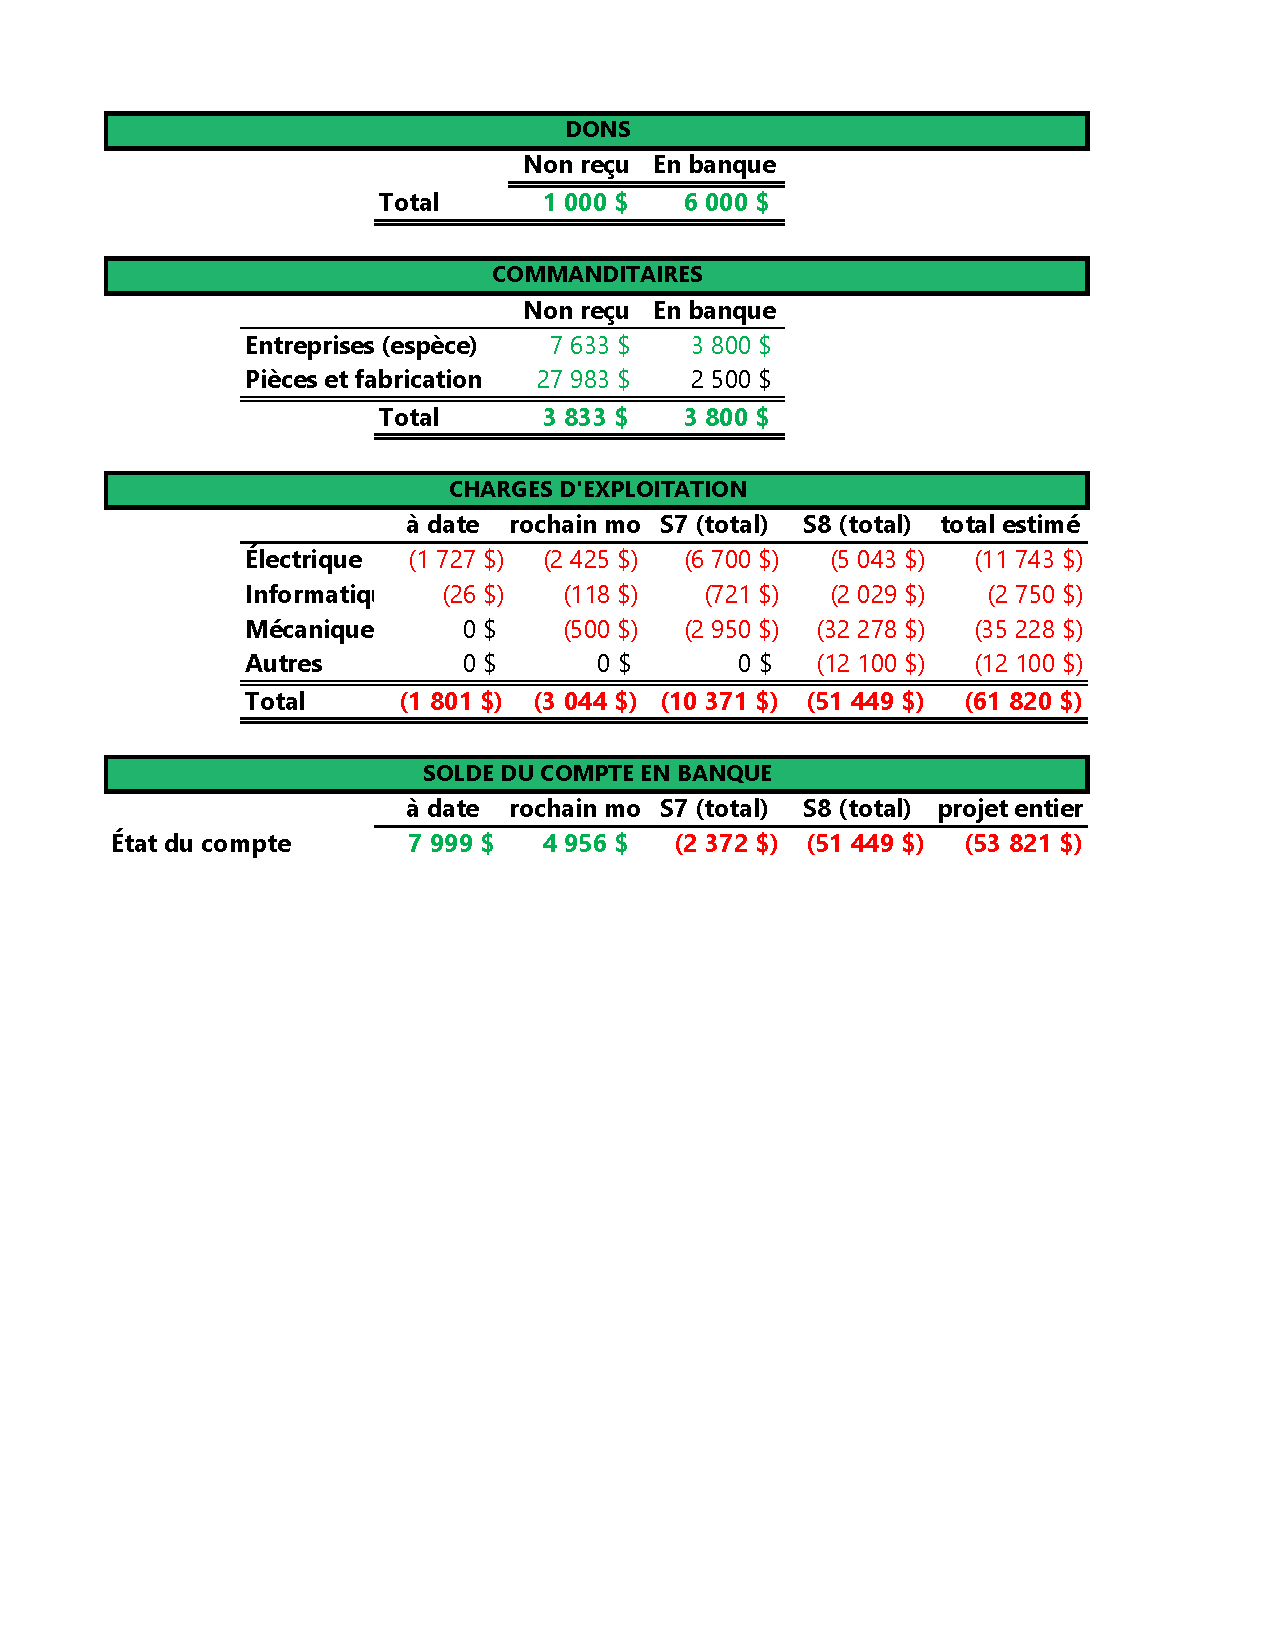
\includegraphics[clip, trim=1.6cm 12cm 4cm 1.6cm, scale=1]{img/argent.pdf}
\end{center}
}
%\hspace{1cm}

\end{poster}

% \begin{poster}
% {
% grid=false,
% headerborder=open, % Adds a border around the header of content boxes
% colspacing=1em, % Column spacing
% bgColorOne=white, % Background color for the gradient on the left side of the poster
% bgColorTwo=white, % Background color for the gradient on the right side of the poster
% borderColor=Mycolor1, % Border color
% headerColorOne=Mycolor2, % Background color for the header in the content boxes (left side)
% headerColorTwo=Mycolor2, % Background color for the header in the content boxes (right side)
% headerFontColor=white, % Text color for the header text in the content boxes
% boxColorOne=white, % Background color of the content boxes
% textborder=rounded, %rectangle, % Format of the border around content boxes, can be: none, bars, coils, triangles, rectangle, rounded, roundedsmall, roundedright or faded
% eyecatcher=false, % Set to false for ignoring the left logo in the title and move the title left
% headerheight=0\textheight, % Height of the header
% headershape=rounded, % Specify the rounded corner in the content box headers, can be: rectangle, small-rounded, roundedright, roundedleft or rounded
% headershade=plain,
% headerfont=\Large\textsf, % Large, bold and sans serif font in the headers of content boxes
% %textfont={\setlength{\parindent}{1.5em}}, % Uncomment for paragraph indentation
% linewidth=1pt % Width of the border lines around content boxes
% }
% {}
% {\textsf{{}}} % Titre vide pcq sinon ça plante
% \hfill \break % Ligne vide pcq sinon ça plante

% \headerbox{Cashflow}{name=cashflow,column=0,span=3}{
% %\vspace{.6cm} % spacing vertical
% %\hspace{1cm}
% \begin{center}
%     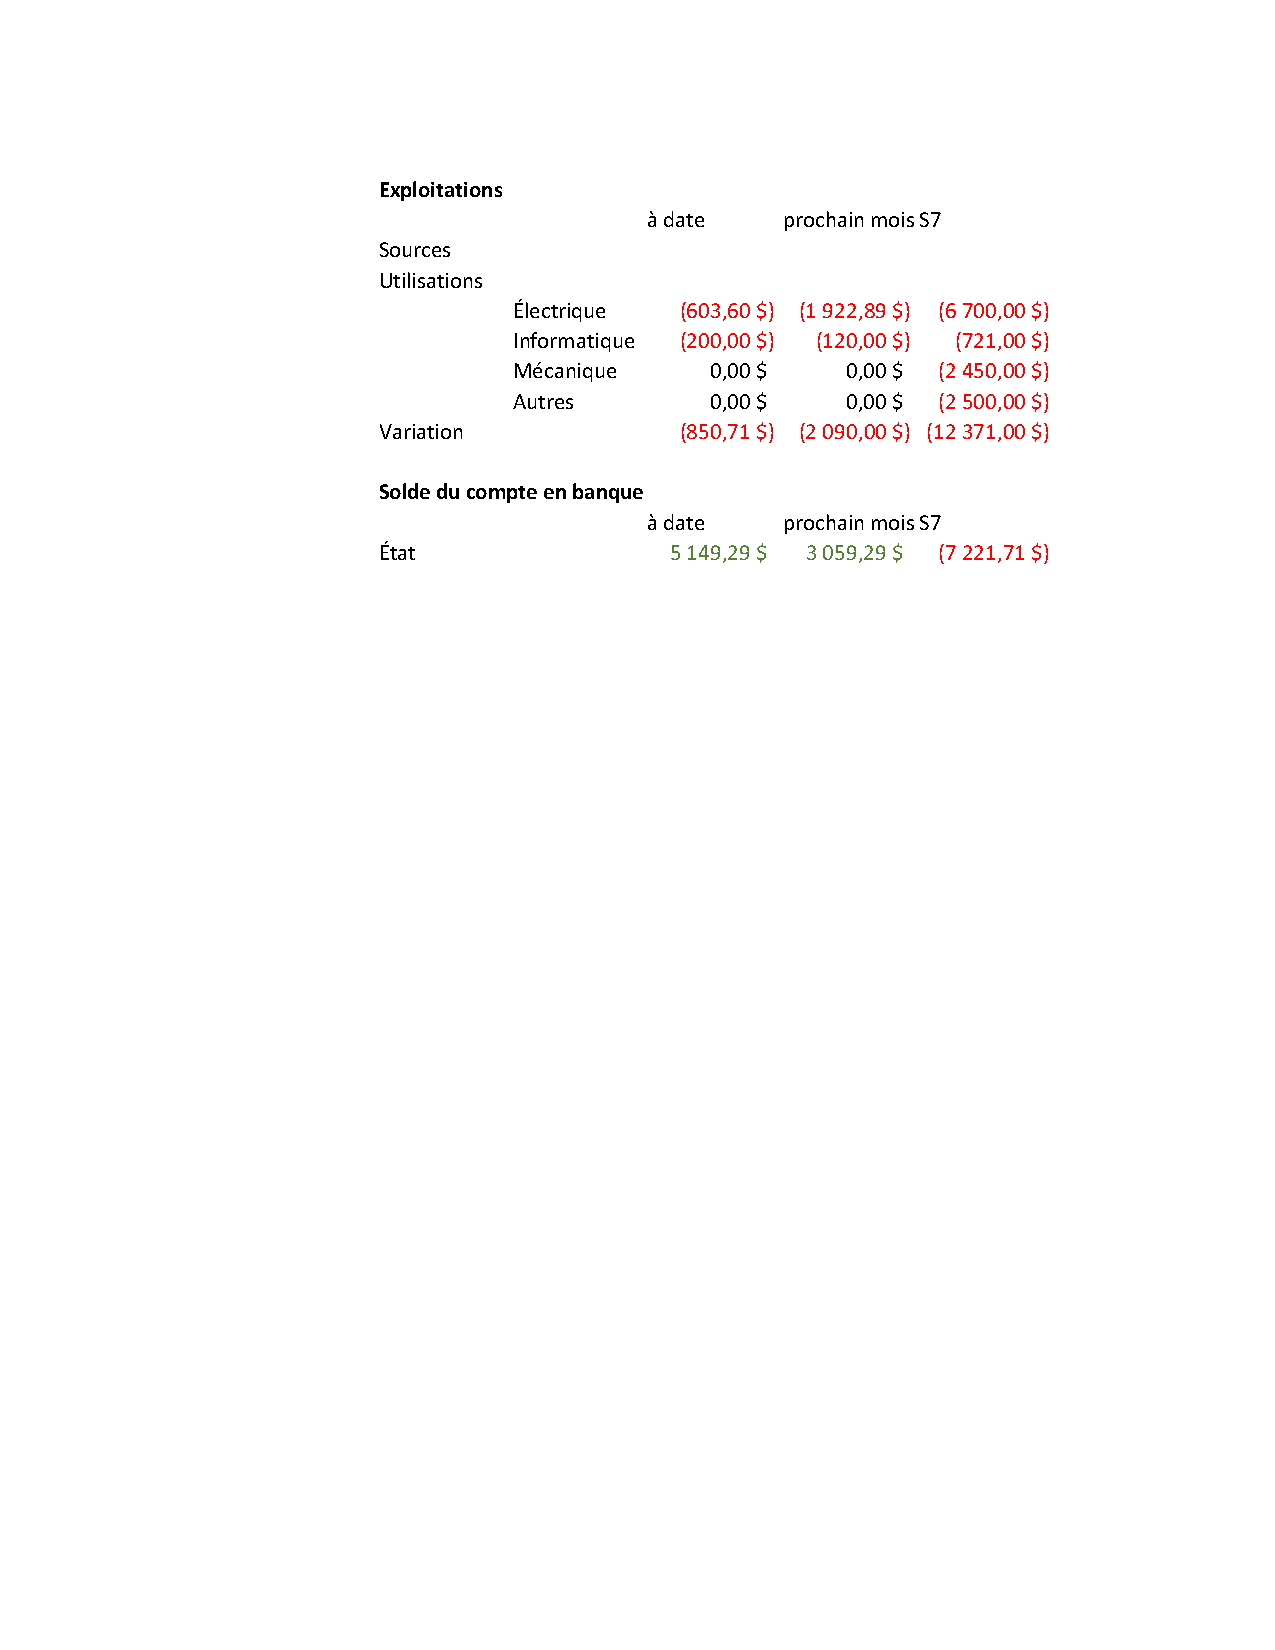
\includegraphics[clip, trim=6cm 17cm 3cm 2cm, scale=1]{img/test.pdf}
% \end{center}
% }

% \end{poster}

\end{document}